% Memoria del Trabajo Fin de Grado del proyecto SavePoint.
% Autor: Felipe Peña Núñez. Escuela Técnica Superior de Ingeniería Informática,
% Universidad de Sevilla. Convocatoria de octubre, curso 2025/2026.

\documentclass[12pt]{report}

% Paquetes LaTeX y estilos globales
\usepackage[utf8]{inputenc}
\usepackage{multicol}
\usepackage{xcolor}
\usepackage{subfigure}
\usepackage[spanish,es-tabla]{babel}
\usepackage{graphicx}
\usepackage{titlesec}
\usepackage[bookmarks,breaklinks,colorlinks=true,allcolors=blue]{hyperref}
\usepackage{listings}
\usepackage{inconsolata}
\usepackage{float}
\usepackage{mathpazo} % Fuente Palatino
\usepackage[labelfont=bf]{caption}

\usepackage[square,numbers]{natbib}
\usepackage[nottoc,notlof,notlot]{tocbibind}  % Mete la bibliografía como capítulo en la TOC, los parámetros excluyen los otros índices de aparecer también
\usepackage{geometry}
\usepackage{amsmath}
\usepackage{parskip}
\usepackage[official]{eurosym}
\usepackage{todonotes}
\usepackage{csquotes}
\usepackage{tocbasic}  % Estilos de la TOC
\usepackage{array}     % Columnas con alineación y ajuste personalizado
\usepackage{tabularx}  % Tablas que se ajustan al ancho de texto disponible

% Formato del título de capítulos y secciones
\titleformat{\chapter}[block]{\normalfont\huge\bfseries}{\thechapter.}{.5em}{\Huge}[\vspace{2pt}{\titlerule[2pt]}]

\titlespacing*{\chapter}{0pt}{-19pt}{25pt}

\titleformat{\section}[block]{\normalfont\Large\bfseries}{\thesection.}{.5em}{\Large}

\titleformat{\part}[block]{\titlerule[2pt]\normalfont\Huge\bfseries\centering}{Parte \Roman{part}\\\vspace{15pt}}{0pt}{\Huge}[\vspace{2pt}{\titlerule[2pt]}]

% Tamaños y estilos de elementos en la TOC
\DeclareTOCStyleEntry[
    linefill=\bfseries\TOCLineLeaderFill,
    beforeskip=12pt,
    entrynumberformat=\chapterprefixintoc,
    entryformat=\chaptertocformat,
    pagenumberformat=\chaptertocformat,
    dynnumwidth
]{tocline}{chapter}

\DeclareTOCStyleEntry[
    % linefill=\bfseries\TOCLineLeaderFill,
    beforeskip=30pt,
    entrynumberformat=\chapterprefixintoc,
    entryformat=\parttocformat,
    pagenumberformat=\partpagetocformat,
    numwidth=0pt
]{tocline}{part}

\newcommand\chaptertocformat[1]{\large{\textbf{#1}}}%
\newcommand\chapterprefixintoc[1]{#1}%
\newcommand\parttocformat[1]{\Large{\textbf{#1}}}%
\newcommand\partpagetocformat[1]{} % Don't print the page number for parts

% Alias para estilos de texto comunes
\newcommand{\negritas}[1]{\textbf{#1}}
\newcommand{\cursiva}[1]{\textit{#1}}
\newcommand{\codigo}[1]{\texttt{#1}}

% Formato del código fuente con lstlisting
\lstset{
  basicstyle=\ttfamily,
  breaklines=true,
}

% Márgenes
\geometry{
    a4paper,
    margin=2.75cm
}
\setlength{\marginparwidth}{2cm} 

% Columnas adaptables para tablas: evitan que los textos largos desborden la página.
\newcolumntype{Y}{>{\raggedright\arraybackslash}X}
\newcolumntype{Z}{>{\centering\arraybackslash}X}
\renewcommand{\tabularxcolumn}[1]{>{\small}m{#1}}
\setlength{\tabcolsep}{4pt}
\renewcommand{\arraystretch}{1.15}

% Tablas compactas y ajustadas al ancho disponible.
\newcommand{\tablecompact}{\small\setlength{\tabcolsep}{3pt}}

% Limite de profundidad del índice
\setcounter{tocdepth}{2}

% Eliminar el guionado
\tolerance=1
\emergencystretch=\maxdimen
\hyphenpenalty=10000
\hbadness=10000

% Indentación de párrafos
\setlength{\parindent}{.75cm}

\renewcommand{\lstlistingname}{Extracto de código}
\renewcommand*{\lstlistlistingname}{Índice de extractos de código}

% Comandos para establecer variables
\newcommand{\setTitle}[1]{\def\tfgTitle {#1}}
\newcommand{\setAuthor}[1]{\def\tfgAuthors {#1}}
\newcommand{\setDegree}[1]{\def\tfgDegree {#1}}
\newcommand{\setSupervisor}[1]{\def\tfgSupervisor {#1}}
\newcommand{\setDepartment}[1]{\def\tfgDepartment {#1}}
\newcommand{\setMonth}[1]{\def\tfgMonth {#1}}
\newcommand{\setYear}[1]{\def\tfgYear {#1}}
\newcommand{\setDedication}[1]{\def\tfgDedication {#1}}

% Estilos para el código
% Configuración genérica
\definecolor{codegreen}{rgb}{0,0.6,0}
\definecolor{codegray}{rgb}{0.5,0.5,0.5}
\definecolor{codepurple}{rgb}{0.58,0,0.82}
\definecolor{editorOcher}{rgb}{0.8, 0.3, 0} % #FF7F00 -> rgb(239, 169, 0)
\definecolor{editorGreen}{rgb}{0, 0.5, 0} % #007C00 -> rgb(0, 124, 0)

\lstdefinestyle{listingstyle}{
    backgroundcolor=\color{white},  
    keywordstyle=\bfseries\color{blue},
    numberstyle=\tiny\color{codegray},
    stringstyle=\color{editorGreen},
    commentstyle=\color{codegray},
    basicstyle=\ttfamily\color{black},
    breakatwhitespace=false,         
    breaklines=true,                 
    captionpos=b,                    
    keepspaces=true,                 
    numbers=left,                    
    numbersep=5pt,                  
    showspaces=false,                
    showstringspaces=false,
    showtabs=false,                  
    tabsize=2,
    frame=tb,
    keywords=[2]{True,False},
    literate=%
*{0}{{{\color{editorOcher}0}}}1
{1}{{{\color{editorOcher}1}}}1
{2}{{{\color{editorOcher}2}}}1
{3}{{{\color{editorOcher}3}}}1
{4}{{{\color{editorOcher}4}}}1
{5}{{{\color{editorOcher}5}}}1
{6}{{{\color{editorOcher}6}}}1
{7}{{{\color{editorOcher}7}}}1
{8}{{{\color{editorOcher}8}}}1
{9}{{{\color{editorOcher}9}}}1,
}

\lstset{style=listingstyle}
\lstset{columns=fullflexible}

\lstdefinelanguage{css}{
  keywords={color,background-image:,margin,padding,font,weight,display,position,top,left,right,bottom,list,style,border,size,white,space,min,width, transition:, transform:, transition-property, transition-duration, transition-timing-function},	
  sensitive=true,
  morecomment=[l]{//},
  morecomment=[s]{/*}{*/},
  morestring=[b]',
  morestring=[b]",
  alsoletter={:},
  alsodigit={-}
}
% JavaScript
\lstdefinelanguage{javascript}{
  morekeywords={abstract, arguments, await, boolean, break, byte, case, catch, char, class, const, continue, debugger, default, delete, do, double, else, enum, eval, export, extends, false, final, finally, float, for, function, goto, if, implements, import, in, instanceof, int, interface, let, long, native, new, null, package, private, protected, public, return, short, static, super, switch, synchronized, this, throw, throws, transient, true, try, typeof, var, void, volatile, while, with, yield},
  morecomment=[s]{/*}{*/},
  morecomment=[l]//,
  morestring=[b]",
  morestring=[b]'
}


%%%%%%%%%%%%%%%%%%%%%%%%%%%%%%%%%%%%%%%%%%%%%%%%%%%%%%%%%%%%%%%%%%%%%%%%%%%%%%%%%%%%%

% Variables para la portada
\setTitle{SavePoint: una plataforma de catalogación de videojuegos como banco de pruebas de algoritmos de recomendación}
\setAuthor{Felipe Peña Núñez}
\setDegree{Grado en Ingeniería Informática - Ingeniería del Software}
\setSupervisor{José Enrique Sánchez López \\ Aitor Rodríguez Dueñas}
\setDepartment{Lenguajes y Sistemas Informáticos}
\setMonth{octubre}
\setYear{2025/2026}

%%%%%%%%%%%%%%%%%%%%%%%%%%%%%%%%%%%%%%%%%%%%%%%%%%%%%%%%%%%%%%%%%%%%%%%%%%%%%%%%%%%%%

% Dedicatoria del trabajo.
\setDedication{A quienes creyeron en este proyecto desde el principio y me acompañaron, con
paciencia y confianza, hasta el final.}

%%%%%%%%%%%%%%%%%%%%%%%%%%%%%%%%%%%%%%%%%%%%%%%%%%%%%%%%%%%%%%%%%%%%%%%%%%%%%%%%%%%%%

% Comienzo del documento
\begin{document}

    % Portada y secciones no numeradas
    \thispagestyle{empty} % Impide que se incluya número de página en la portada
\begin{center}

\vspace*{1cm}


\includegraphics[width=\textwidth]{figures/etsii_us.png}

\vspace*{3cm}
\begin{large}
TRABAJO FIN DE GRADO
\end{large}

\vspace*{0.1in}
\textbf{\huge \tfgTitle}

\vspace*{.2in}

{\large Realizado por}\\
\textbf{\Large \tfgAuthors}

\vspace*{3cm}

\textbf{Para la obtención del título de}\\
{\large \tfgDegree}

\vspace*{0.2in}

\textbf{Dirigido por}\\
{\large \tfgSupervisor}\\

\vspace*{0.2in}

\textbf{En el departamento de}\\
{\large \tfgDepartment}

\vspace*{.6in}
\textbf{\Large Convocatoria de \tfgMonth, curso \tfgYear}

\end{center}

% Dedicatoria. La página se mantiene activa con texto provisional visible; el
% autor la redactará antes de la entrega final.
\ifdefined\tfgDedication
    \newpage
    \thispagestyle{empty}

    \vspace*{\fill}
    \begin{center}
    \textit{\tfgDedication}
    \end{center}
    \todo[inline]{Dedicatoria pendiente de completar antes de la entrega.}
    \vspace*{\fill}
\fi

\clearpage\setcounter{page}{1} % Comienza a incluir números de página a partir de aquí
\pagenumbering{roman} % En números romanos

    \chapter*{Agradecimientos}
\addcontentsline{toc}{chapter}{Agradecimientos}

Esta sección se completará antes de la entrega final.

\todo[inline]{Agradecimientos pendientes: el autor añadirá a los tutores, a la familia y a los compañeros que han acompañado el desarrollo del proyecto.}

    \chapter*{Resumen}
\addcontentsline{toc}{chapter}{Resumen}

SavePoint nace de aplicar al videojuego el patrón de catalogación personal de plataformas como Goodreads o Letterboxd, con un inventario de propiedad física y digital que esos productos no necesitan resolver; sobre esa base, el trabajo convierte la plataforma en un banco de pruebas reproducible para sistemas de recomendación. Se ha diseñado e implementado el producto con catálogo, biblioteca, copias físicas y digitales, valoraciones, listas, comentarios, perfiles, privacidad, relaciones sociales y recomendaciones. La aplicación y la evaluación reproducible de los recomendadores son las dos partes complementarias del trabajo: la primera recoge y gobierna los datos que la segunda necesita.

El sistema compara dieciséis algoritmos de referencia: baselines, variantes basadas en contenido, filtrado colaborativo por vecinos e híbridos con reordenación por diversidad. Se describen la representación de obras y perfiles, la ponderación de etiquetas, la similitud por facetas, la calidad externa, la popularidad, la evidencia negativa, el arranque en frío y la combinación híbrida. El protocolo offline fija corpus, snapshots, semillas, candidatas comunes, exclusiones y métricas para $K\in\{5,10,20\}$.

La evidencia publicada v15 utiliza 400 usuarios sintéticos activos y 79 usuarios evaluables, con una sola ejecución del test. Los resultados permiten comparar internamente algoritmos bajo el corpus y protocolo congelados, pero no representan usuarios reales ni justifican generalizaciones automáticas. La memoria distingue de forma explícita esa publicación del contrato de implementación vigente, que evolucionó posteriormente.

Se ha aplicado una metodología de ingeniería asistida por agentes, gobernada mediante el método Get Stuff Done y organizada conceptualmente con Obsidian. Las herramientas se emplearon bajo dirección y revisión humana, manteniéndose la decisión final y la responsabilidad sobre el análisis, el diseño, la implementación y la validación en la dirección del proyecto. La trazabilidad entre requisitos, código, pruebas, decisiones y artefactos versionados constituye una aportación metodológica del trabajo.

\vspace{.5cm}
\textbf{Palabras clave:} videojuegos, sistemas de recomendación, evaluación offline, reproducibilidad, filtrado colaborativo, recomendación basada en contenido, procedencia de datos.

    \chapter*{Abstract}
\addcontentsline{toc}{chapter}{Abstract}

SavePoint grew out of applying to video games the personal cataloguing pattern of platforms such as Goodreads or Letterboxd, adding an inventory of physical and digital ownership that those products never had to solve; on that basis, the project turns the platform into a reproducible testbed for recommender systems. The platform includes a catalogue, library, physical and digital copies, ratings, lists, comments, profiles, privacy, social relations and recommendations. The application and the reproducible evaluation of the recommenders are the two complementary halves of the work: the former collects and governs the data the latter needs.

The system compares sixteen reference algorithms: baselines, content-based variants, neighbourhood collaborative filtering, and hybrid approaches with diversity re-ranking. This report describes item and user representations, tag weighting, facet similarity, external quality, popularity, negative evidence, cold start, and hybrid combination. The offline protocol fixes corpus, snapshots, seeds, shared candidates, exclusions and ranking metrics at $K\in\{5,10,20\}$.

The published v15 evidence uses 400 active synthetic users and 79 evaluable users, with a single test run. It supports an internal comparison under the frozen corpus and protocol, but it does not represent real users or justify automatic generalisation. This report explicitly separates that publication from the later implementation contract.

An agent-assisted engineering methodology governed through the Get Stuff Done method and conceptually organised with Obsidian was applied throughout the project. The tools were used under human direction and review, while final decisions and responsibility for analysis, design, implementation and validation remained with Felipe Peña Núñez.

\vspace{.5cm}
\textbf{Keywords:} video games, recommender systems, offline evaluation, reproducibility, collaborative filtering, content-based recommendation, data provenance.

    \chapter*{Acrónimos}
\addcontentsline{toc}{chapter}{Acrónimos}

La siguiente lista recoge los acrónimos empleados en la memoria. Cada uno se define también
en su primer uso dentro del cuerpo del texto, con la forma larga seguida de la sigla. En el
resumen y en el \textit{abstract} se han escrito las formas largas, sin siglas.

\begin{description}
    \item[ADR] Registro de decisión de arquitectura (del inglés \textit{architecture decision record}).
    \item[API] Interfaz de programación de aplicaciones (del inglés \textit{application programming interface}).
    \item[CC0] Dedicación al dominio público \textit{Creative Commons Zero}.
    \item[CDN] Red de distribución de contenidos (del inglés \textit{content delivery network}).
    \item[CSRF] Falsificación de petición en sitios cruzados (del inglés \textit{cross-site request forgery}).
    \item[CSV] Valores separados por comas (del inglés \textit{comma-separated values}).
    \item[DLC] Contenido descargable (del inglés \textit{downloadable content}).
    \item[DoS] Denegación de servicio (del inglés \textit{denial of service}).
    \item[DRF] \textit{Django REST Framework}.
    \item[DSA] Acuerdo de servicios para desarrolladores (del inglés \textit{developer services agreement}).
    \item[DTO] Objeto de transferencia de datos (del inglés \textit{data transfer object}).
    \item[E2E] De extremo a extremo (del inglés \textit{end to end}).
    \item[GSD] \textit{Get Stuff Done}, método de desarrollo dirigido por especificación para agentes.
    \item[HTTP] Protocolo de transferencia de hipertexto (del inglés \textit{hypertext transfer protocol}).
    \item[IGDB] \textit{Internet Game Database}.
    \item[JSON] Notación de objetos de JavaScript (del inglés \textit{JavaScript object notation}).
    \item[LTS] Soporte a largo plazo (del inglés \textit{long-term support}).
    \item[ML] Aprendizaje automático (del inglés \textit{machine learning}).
    \item[nDCG] Ganancia acumulada descontada y normalizada (del inglés \textit{normalized discounted cumulative gain}).
    \item[ORM] Mapeo objeto-relacional (del inglés \textit{object-relational mapping}).
    \item[PaaS] Plataforma como servicio (del inglés \textit{platform as a service}).
    \item[REST] Transferencia de estado representacional (del inglés \textit{representational state transfer}).
    \item[SSR] Renderizado en el servidor (del inglés \textit{server-side rendering}).
    \item[TFG] Trabajo Fin de Grado.
    \item[UAT] Pruebas de aceptación de usuario (del inglés \textit{user acceptance testing}).
    \item[UI] Interfaz de usuario (del inglés \textit{user interface}).
    \item[UUID] Identificador único universal (del inglés \textit{universally unique identifier}).
    \item[WCAG] Pautas de accesibilidad para el contenido web (del inglés \textit{web content accessibility guidelines}).
    \item[XSS] Ejecución de secuencias de comandos en sitios cruzados (del inglés \textit{cross-site scripting}).
\end{description}


    % Índice del documento y de figuras
    \begingroup
        % Los enlaces son normalmente azules, pero en los índices se configuran a negro para que no aparezca todo azul
        \hypersetup{linkcolor=black}
        \tableofcontents
        \listoffigures
        \listoftables
        \lstlistoflistings
    \endgroup

    % Cambia el estilo de números de página de romanos a normal
    \clearpage\pagenumbering{arabic}

    % Capítulos del trabajo
    \part{Introducción y planificación}\label{part:introduccion}
    \chapter{Introducción, problema y objetivos}\label{cap:introduccion}

\section{Motivación, contexto y problema}\label{sec:origen-motivacion}\label{sec:contexto-problema}\label{sec:arte-productos}\label{sec:arte-aportacion}

Goodreads y Letterboxd son dos servicios web de catalogación social: el primero, para libros,
y el segundo, para cine~\cite{goodreads,letterboxd}. Ambos comparten un patrón: una ficha canónica
por obra, independiente de la edición concreta que posea cada persona; un estado de consumo
personal, como pendiente, en curso o terminado; una valoración con una escala consistente;
listas ordenadas. Ni uno ni
otro representan la propiedad material con detalle, porque un libro o una película no plantean
el problema de inventario que sí plantea una consola con juegos en cartucho, disco y descarga.

En el ámbito del videojuego, Backloggd traslada casi literalmente el modelo de
Letterboxd~\cite{backloggd}, con buen tratamiento del backlog, pero sin inventario de
copias ni ambición de recomendación. OpenCritic agrega puntuaciones de prensa y es una
referencia de densidad visual y de tratamiento de la nota, más que un catalogador personal.
Steam ofrece una biblioteca personal rica, aunque acoplada a su tienda y limitada a lo
comprado en ella. La web de IGDB expone un catálogo amplio y bien modelado, orientado a la
consulta y no a la gestión de una colección. La Tabla~\ref{tab:productos} resume la comparación.

\begin{table}[htp]
\centering
\begin{tabularx}{\textwidth}{ | L{0.18\textwidth} | Z | Z | Z | Z | }
    \hline
    \textbf{Producto} & \textbf{Ficha canónica} & \textbf{Backlog} & \textbf{Inventario de copias} & \textbf{Recomendación} \\
    \hline
    Goodreads & Sí & Sí & No & Sí \\
    \hline
    Letterboxd & Sí & Sí & No & Parcial \\
    \hline
    Backloggd & Sí & Sí & No & No \\
    \hline
    OpenCritic & Sí & No & No & No \\
    \hline
    Steam & Parcial & Parcial & Solo digital de su tienda & Sí \\
    \hline
    IGDB.com & Sí & No & No & No \\
    \hline
    \textbf{SavePoint} & Sí & Sí & Sí & Sí \\
    \hline
\end{tabularx}
\caption{Comparación de SavePoint con los productos de referencia.}
\label{tab:productos}
\end{table}

El hueco que SavePoint ocupa se ve en la última columna de la
Tabla~\ref{tab:productos}: ningún producto reúne un inventario detallado de propiedad
material con un catálogo a escala real y un banco de pruebas de recomendación abierto y
reproducible. Es un problema propio del videojuego: un mismo título puede poseerse a la vez en
cartucho, en disco y en descarga, y en más de una plataforma, una distinción que no tiene ficha
ni equivalente en un libro o una película.

SavePoint se propone cubrir ese hueco. Aplica al videojuego el patrón de catalogación personal
de Goodreads y Letterboxd, con ficha canónica de cada obra, biblioteca, valoraciones y relaciones
de amistad, y añade lo que esos productos no necesitan y este medio sí: un inventario de copias
físicas y digitales por edición y plataforma, con procedencia de datos verificable en lugar de
un catálogo mantenido a mano. De ello se desprenden tres aportaciones. La primera es un
producto de catalogación de videojuegos que combina inventario de propiedad material, catálogo
a escala real y procedencia de datos documentada, un conjunto que ningún servicio existente
reúne, como muestra la Tabla~\ref{tab:productos}. La segunda es un banco de pruebas reproducible
para la comparación de recomendadores, con corpus citable, usuarios sintéticos y procedencia de
datos documentada, que se explota mediante un protocolo de evaluación congelado y una
comparación real entre dieciséis algoritmos, presentada en el Capítulo~\ref{cap:resultados}. La
tercera es la propia metodología de ingeniería asistida por agentes, aplicada de forma
sistemática y versionada en el repositorio, de manera que el proceso que produjo el sistema es
tan inspeccionable y reproducible por un tercero como el sistema mismo; el
Capítulo~\ref{cap:gestion} la desarrolla en profundidad.

El trabajo es, ante todo, un desarrollo de ingeniería del software: el diseño, la construcción,
la verificación y el despliegue de una plataforma web completa para catalogar videojuegos,
mantener una biblioteca personal y registrar valoraciones, listas, copias, comentarios y
relaciones sociales. El módulo de recomendación y su evaluación forman parte de esa
plataforma y tienen el mismo peso que el resto: sin un catálogo gobernado y una biblioteca con
señales reales no hay nada que recomendar, y sin una evaluación reproducible no hay forma
honesta de saber si lo recomendado funciona. La plataforma recoge y gobierna las señales que
los algoritmos consumen, y el laboratorio compara esos algoritmos sobre los mismos datos.

Una lista de recomendaciones no es evidencia suficiente de que un algoritmo funciona mejor que
otro. Sin un corpus congelado, una población definida, una división conocida y artefactos
identificables, dos ejecuciones pueden parecer comparables aunque en realidad respondan a
experimentos distintos, con datos distintos o con criterios de éxito distintos. SavePoint
separa por ello, de forma deliberada, la aplicación que presenta resultados a un usuario de los
trabajos offline que construyen y evalúan esos rankings. Esa separación no es solo una decisión
de arquitectura: se diseñó, implementó y validó mediante código, pruebas y evidencias
versionadas. Es esa separación la que permite que las conclusiones del
Capítulo~\ref{cap:resultados} de esta memoria se puedan volver a comprobar.

\section{Objetivos y alcance}\label{sec:objetivos}\label{sec:alcance-limites}

El objetivo general del trabajo es construir una plataforma de catalogación de videojuegos que
sirva, al mismo tiempo, como banco de pruebas reproducible para recomendación basada en
contenido, colaborativa e híbrida. De ahí se derivan las cuestiones que el trabajo
aborda: qué señales de un videojuego (género, plataforma, etiquetas curadas, calidad
externa, popularidad) se pueden representar de forma explicable en un catálogo real; cómo
cambia la recuperación de un ítem relevante cuando se combinan contenido, popularidad,
vecindad entre usuarios y diversidad de la lista resultante; y qué conclusiones son
defendibles cuando el corpus y la población de usuarios son, como se explica más abajo,
sintéticos y no personas reales.

Los objetivos específicos son gobernar el catálogo y su procedencia de datos; modelar
biblioteca, privacidad y relaciones sociales con el mismo nivel de cuidado que el catálogo;
implementar tanto los algoritmos de referencia (\textit{baselines}) como las tres familias de
recomendación descritas en el Capítulo~\ref{cap:estado-del-arte}; publicar un protocolo offline
con candidatas comunes para que la comparación entre algoritmos sea justa; y conservar hashes,
configuraciones y artefactos que hagan auditable cada resultado. La expectativa de partida del
trabajo no afirma la superioridad universal de ningún algoritmo: bajo el protocolo publicado,
combinar señales de contenido, popularidad y vecindad puede mejorar la recuperación frente a
los baselines más simples, pero esa mejora debe contrastarse sin confundir una diferencia
numérica con significación estadística o con validez fuera del corpus y la población con los
que se midió.

El alcance funcional del producto incluye catálogo, importación gobernada de datos, biblioteca,
copias físicas y digitales, valoraciones, listas, comentarios, perfiles, privacidad, módulo
social, recomendaciones y las medidas de seguridad y copia de
seguridad propias de un servicio con usuarios. De las dieciséis variantes de recomendación
evaluadas, la aplicación publica tres, según se explica en la
Sección~\ref{sec:alg-publicadas}. El alcance de la evaluación, en cambio, se limita a
una publicación de evidencia concreta, identificada como v15 y descrita en el
Capítulo~\ref{cap:resultados}, con una única ejecución del test. Conviene subrayar que estos usuarios sintéticos no son personas
reales, sino perfiles generados de forma controlada para poder ejercitar el sistema de
recomendación sin depender de una base de usuarios real que este TFG no tiene tiempo ni alcance
para reunir. Los resultados, por tanto, dependen del corpus concreto, de la semilla aleatoria,
de la división de datos y del protocolo empleados: no permiten generalizar automáticamente a
preferencias de jugadores reales ni declarar un método como mejor fuera de esas condiciones.

\section{Estructura de la memoria}\label{sec:estructura-memoria}

La memoria sigue el recorrido natural de un proyecto de ingeniería del software, tratando la
plataforma y el estudio de recomendadores en un único hilo. El
Capítulo~\ref{cap:estado-del-arte} revisa las fuentes de datos, los sistemas de
recomendación y su evaluación, y el método de trabajo. El Capítulo~\ref{cap:gestion} describe la
gestión, la metodología y la planificación del trabajo, con su calendario, su presupuesto y sus
riesgos. El Capítulo~\ref{cap:analisis} recoge el análisis del problema: actores, requisitos de
la plataforma y de la evaluación de recomendadores, reglas de negocio y trazabilidad. El
Capítulo~\ref{cap:diseno} presenta el diseño y la arquitectura, incluidos los algoritmos de
recomendación con sus fórmulas y ponderaciones. El Capítulo~\ref{cap:implementacion} describe la
implementación, los datos, las pruebas y el despliegue. El Capítulo~\ref{cap:resultados}
somete las dieciséis variantes al protocolo de evaluación y presenta los resultados. El
Capítulo~\ref{cap:conclusiones} cierra con el grado de cumplimiento de los objetivos, las
limitaciones y las líneas de continuación.

    \chapter{Gestión y metodología de trabajo}\label{cap:gestion}

El autor organizó SavePoint en siete fases, desde catálogo y biblioteca hasta la comparación experimental y la preparación de demostración. La planificación se conserva en \texttt{PROJECT.md}, \texttt{REQUIREMENTS.md}, \texttt{ROADMAP.md}, \texttt{STATE.md}, planes, resúmenes y verificaciones. Esta cadena permite enlazar una decisión con un cambio, una prueba y su evidencia; la matriz de trazabilidad conserva los detalles sin sobrecargar la memoria principal.

El autor aplicó una metodología de ingeniería asistida por agentes, gobernada mediante GSD y organizada conceptualmente con Obsidian. El ciclo de discutir, investigar, planificar, ejecutar y verificar conserva contexto entre tareas. Los agentes se emplearon como herramientas para planificar, investigar, revisar, auditar y generar propuestas; el autor revisó, modificó o rechazó esas propuestas y asumió todas las decisiones y la responsabilidad académica. El vault enlaza conceptos, fases y ADR con fuentes canónicas, pero no sustituye tests, hashes ni artefactos versionados.

La metodología reduce pérdida de contexto y facilita reanudación, pero no garantiza corrección. Depende de especificaciones claras, requiere revisión humana y puede dejar documentación desactualizada. \todo[inline]{PENDIENTE: incorporar horas, calendario y presupuesto con el registro que el autor considere defendible.}


    \part{Núcleo I: Investigación y algoritmos de recomendación}\label{part:nucleo-investigacion}
    \chapter{Antecedentes y estado del arte}\label{cap:estado-del-arte}

\todo[inline]{Capítulo por redactar en la siguiente iteración.}

    \chapter{Algoritmos de recomendación y representación de señales}\label{cap:algoritmos}

\section{Frontera temporal de la comparación}

Este capítulo distingue dos contratos. Los resultados publicados proceden de la ejecución \texttt{evaluation-400-test-2026-09-12-v15}, con protocolo 15 y \textit{feature set} \texttt{fs-v12-curated-tags-idf}. El código vigente evolucionó después al protocolo 16 y a \texttt{fs-v13-family-weighted-tags}. La evolución permite describir la implementación actual, pero no recalcula ni reinterpreta las métricas v15. Esta distinción evita atribuir a una publicación histórica pesos o fórmulas posteriores.

La comparación v15 contiene dieciséis variantes: \texttt{random-v1}, \texttt{popularity-v1}, diez variantes de contenido, dos variantes con MMR, \texttt{cf-user-knn-v1}, \texttt{hybrid-weighted-cf-v1} y \texttt{hybrid-mmr-v1}. El sistema también expone \texttt{tag-taste-v1} como heurística de producto; no pertenece a la comparación académica porque resuelve onboarding, no una hipótesis experimental comparable.

\section{Datos, elegibilidad y perfil}

Una candidata debe ser una obra gobernada del corpus, no DLC, publicada antes de la fecha de corte, con valoración externa disponible y al menos cinco valoraciones. También se excluye cualquier obra que ya aparezca en \texttt{LibraryEntry} de la persona. Estas exclusiones impiden recomendar una posesión conocida, lanzar contenido futuro o amplificar una nota con evidencia insuficiente.

Cada obra se representa mediante un vector disperso de familias de facetas. En el contrato actual, los géneros y subgéneros curados forman el núcleo semántico; tema, característica, modo, franquicia y desarrollador actúan como confirmaciones opcionales; la plataforma expresa compatibilidad material. Las \emph{keywords}, perspectivas y modos crudos no se introducen directamente: su ruido y heterogeneidad se reducen previamente mediante curación editorial. Una faceta ausente se omite; no se imputa ni redistribuye su peso.

Para un término \(t\) de una familia \(f\), la ponderación usa una frecuencia documental inversa suavizada:

\begin{equation}\label{eq:idf}
idf(t)=\ln\left(\frac{N_f+1}{df_t+1}\right)+1,
\end{equation}

donde \(N_f\) es el número de obras gobernadas con algún valor de la familia y \(df_t\) el número que contiene \(t\). Si \(T\) es el conjunto de valores de una obra, el peso de la coordenada es \(w(f:t)=W_f\,idf(t)/\sqrt{\sum_{q\in T}idf(q)^2}\). La normalización L2 evita que una obra gane afinidad solo por declarar más etiquetas. Los pesos \(W_f\), el suavizado y la taxonomía son decisiones de SavePoint, no parámetros universales.

El perfil positivo combina obras terminadas o en curso con valoración personal suficiente. Para una entrada \(i\), \(status\_weight\) vale 3 para terminada, 2 para en curso, 1 para pendiente y 0 para abandonada. Si \(r\) es la valoración personal normalizada, la intensidad es \(r^2\); por tanto, \(entry\_weight_i=status\_weight_i+r_i^2\). El perfil se obtiene como media ponderada de los vectores normalizados de las entradas elegibles. Las valoraciones inferiores al umbral aportan evidencia negativa solo cuando una etiqueta se repite en al menos tres experiencias negativas. Esta salvaguarda evita inferir un rechazo estable a partir de una sola obra.

\section{Similitud y puntuación de contenido}

La similitud principal no aplica coseno ciegamente a todo el vector. Para cada familia se calcula cobertura del perfil y precisión de la candidata. Sean \(P_f\) y \(C_f\) sus valores, y \(O_f=P_f\cap C_f\). Entonces \(coverage_f=\sum_{t\in O_f}P_f[t]/\sum_{t\in P_f}P_f[t]\) y \(precision_f=|O_f|/|C_f|\). Ambas cantidades se combinan mediante \(F_{0.5}\):

\begin{equation}\label{eq:fbeta}
F_{0.5}=\frac{(1+0.5^2)\,coverage\,precision}{0.5^2\,precision+coverage}.
\end{equation}

El parámetro menor que uno prioriza que la candidata no acumule facetas irrelevantes. El núcleo combina las familias activas de género y plataforma por media ponderada. Tema, característica, modo, franquicia y desarrollador solo añaden un bono acotado cuando confirman una coincidencia; su ausencia es neutral. La similitud se limita a \([0,1]\). El coseno se reserva para la redundancia entre recomendaciones y la diversidad intra-lista, donde su interpretación geométrica es directa.

La variante \texttt{content-cbf-weighted-v1} usa la suma ponderada de afinidad y calidad externa. Las variantes multiplicativas, de dos etapas y negativas modifican respectivamente la combinación con rating, el desempate dentro de una banda de similitud y la penalización por perfil negativo. Las variantes \texttt{-pop-v1} incorporan además PopScore normalizado. \texttt{recency-v1} añade recencia como señal explícita. Ninguna de estas variantes cambia el conjunto común de candidatas.

La calidad externa se estabiliza con \emph{shrinkage} bayesiano. Con \(n\) valoraciones, prior del corpus \(\mu\) y \(m=25\), se usa \(rating_{bayes}=(n\,rating+m\,\mu)/(n+m)\), seguido de una confianza \(n/(n+m)\). Así, una nota extrema con pocas observaciones queda contraída hacia el corpus. PopScore se transforma con \(\log(1+x)\) y percentil de rango dentro del snapshot congelado, no con el valor bruto.

\section{Colaborativo, híbrido y diversidad}

\texttt{cf-user-knn-v1} compara valoraciones explícitas de usuarios mediante vecindad. La similitud se calcula sobre obras co-valoradas, exige al menos dos coincidencias y conserva vecinos positivos hasta un máximo de 20. Su predicción agrega la desviación de cada vecino respecto a su media, ponderada por similitud. Es explicable por los vecinos y las obras compartidas, pero sufre \emph{cold start}: con historial escaso o sin vecindad suficiente no puede inferir preferencia colaborativa fiable.

El híbrido ponderado combina las dos fuentes como \(H(i)=0.60\,ContentWeighted(i)+0.40\,CF(i)\). Si el componente colaborativo no dispone de historial, conserva la relevancia de contenido y declara el \emph{fallback}; no penaliza artificialmente a un usuario nuevo. El peso 0.60/0.40 es una decisión local que debe evaluarse, no una regla derivada de la literatura.

Las variantes MMR reordenan un pool de tamaño \(\max(100,5K)\). En cada posición seleccionan la candidata que maximiza \(\lambda\,Rel(i)-(1-\lambda)\max_{j\in S}cosine(i,j)\), con \(\lambda=0.80\). \(Rel(i)\) es la relevancia previa y \(S\) la lista ya elegida. La penalización no cambia el score base ni garantiza mejor precisión: hace visible el intercambio entre relevancia y redundancia.

\section{Limitaciones y alternativas}

Las familias implementadas son interpretables y adecuadas para una población controlada, pero no agotan el espacio de recomendación. No se adoptaron microservicios, Kafka ni Kubernetes por complejidad operativa injustificada en v1; tampoco base vectorial, entrenamiento en HTTP, SQLite en producción o evaluación contra APIs vivas, porque perjudicarían reproducibilidad o integridad. Se descartaron factorización matricial, redes neuronales y recomendadores profundos por requerir más interacciones, entrenamiento e hiperparámetros de los que permite defender esta población sintética. Son decisiones de alcance, no una afirmación de inferioridad universal.


    \part{Núcleo II: Aplicación web}\label{part:nucleo-web}
    \chapter{Aplicación web}\label{cap:diseno}

Este capítulo reúne todo lo que corresponde al producto: qué debe hacer, cómo se diseñó, cómo
se construyó y dónde se despliega. Recorre, en un único hilo, los requisitos que fijan el
alcance, la arquitectura y el modelo de datos que le dan forma, la implementación que los
materializa y la topología pública en la que se sirve, de modo que el lector no tenga que
saltar entre capítulos para reconstruir una sola pieza del sistema. El Capítulo~\ref{cap:nucleo-investigacion}
recoge, por separado, el otro núcleo del trabajo: los algoritmos de recomendación y su
evaluación, que se apoyan en esta misma plataforma pero se estudian con su propio rigor
experimental.

\section{Análisis de requisitos}\label{cap:requisitos}

El sistema distingue tres actores con acceso real. El visitante, sin autenticar, puede
consultar el catálogo, la ficha de cada juego con su procedencia, un perfil público y la
recomendación por popularidad. La persona usuaria, titular de una cuenta controlada, gestiona
además su propia lista de pendientes, valora juegos e inventaría sus copias físicas y
digitales. La cuenta simulada es una variante etiquetada con claridad como tal, precargada
para que el tribunal y cualquier visitante puedan recorrer el sistema sin crear una cuenta
propia. Dos actores adicionales, un perfil de administración de cuentas y catálogo y un perfil
de personal investigador con acceso al panel de comparación de algoritmos, se incluyen en el
análisis para dar contexto completo al modelo, aunque su implementación queda fuera del
alcance descrito en esta memoria.

El modelo de dominio distingue tres áreas: catálogo, biblioteca personal y cuentas. En el
catálogo, la entidad central es la obra (\texttt{GameWork}), la identidad canónica de un
título de videojuego con independencia de la plataforma y de la edición concreta, con un
identificador único universal (UUID) generado en el momento de la importación, de modo que
cambiar de proveedor de enriquecimiento, o prescindir de él, nunca obliga a renumerar el
catálogo. Cada obra puede tener varias publicaciones, una por plataforma; cada publicación
puede tener a su vez varias ediciones. La obra guarda también, de forma deliberadamente
desnormalizada, la fecha de primer lanzamiento y la valoración agregada de origen, para que
filtrar por año o por nota sea un recorrido de índice y no una agregación sobre cientos de
miles de publicaciones en cada consulta, y los alias bilingües sostienen la búsqueda tolerante
a errores tipográficos mediante un índice de trigramas. La procedencia de cada obra (fuente,
identificador de origen, licencia, fecha de recuperación y huella del contenido) se conserva
junto a ella, no como un metadato aparte que se pueda perder. En la biblioteca personal, la
entrada de biblioteca representa la relación entre una persona y una obra: su estado en la
lista de pendientes y su valoración, esta última almacenada como un entero de medias estrellas
entre uno y diez, nunca como un número en coma flotante que introduciría precisión falsa, con
una restricción de unicidad que impide más de una entrada por persona y obra. El historial de
cambios de estado se conserva como un registro de solo anexado, de forma que se puede
reconstruir cuándo una persona empezó, dejó o retomó un juego, y las copias en propiedad
representan cada ejemplar físico o digital, con su formato, su publicación y su edición, y una
clave de idempotencia que evita duplicados cuando el usuario reintenta un alta que en realidad
ya se había registrado. En cuentas, el sistema usa el modelo de usuario de Django directamente
y añade sobre él las entidades necesarias para identificar de forma inequívoca qué cuentas son
simuladas, con una restricción de base de datos que impide, incluso por error de aplicación,
que una cuenta simulada deje de estar marcada como tal.

De los noventa y cuatro requisitos identificados en el análisis, noventa y dos están
completos, con evidencia verificable en \texttt{docs/verification/} o en las firmas de
aceptación por fase. Entre los completos están la autenticación con cuentas simuladas, la
búsqueda y el filtrado del catálogo, la ficha de detalle con su procedencia, el ciclo completo
de biblioteca y copias, la portabilidad de la colección (exportación versionada y una
importación validada con previsualización, errores fila a fila y reglas deterministas de
conflicto), la privacidad de perfil y, como desarrolla en profundidad el
Capítulo~\ref{cap:nucleo-investigacion} de esta memoria, las tres familias completas de
recomendación con su protocolo de evaluación offline, incluidas sus métricas de precisión,
cobertura, diversidad y novedad por cohorte de usuario. Los dos requisitos que quedan
pendientes son parciales, no partidas sin empezar, y ambos pertenecen al mismo contrato de
evaluación: repetir la comparación de algoritmos con varias semillas, más allá de la ejecución
única ya publicada como v15, y retroproyectar sobre esa misma ejecución histórica la captura de
entorno y consumo de recursos que el ejecutor paralelo ya sabe registrar para comparaciones
futuras. Ambos quedan documentados como líneas de continuación explícitas en el
Capítulo~\ref{cap:conclusiones}, no presentados como si ya existieran.

Los requisitos no funcionales se agrupan en cinco familias. La reproducibilidad exige que el
sistema arranque de forma determinista en un entorno local documentado, con todas las
dependencias fijadas a una versión exacta. La legalidad y procedencia de datos exige que cada
dato del catálogo conserve su fuente, su licencia y su fecha de recuperación, con la elección
de cada fuente documentada junto con sus términos de uso. La accesibilidad y el diseño
responsive exigen que los flujos principales funcionen con teclado y en anchuras de
escritorio y de móvil, verificables frente a las Pautas de Accesibilidad para el Contenido Web
(WCAG) 2.2 en nivel AA~\cite{wcag22}. La seguridad de la demostración controlada exige que
ningún secreto aparezca en el control de versiones, en los paquetes servidos al navegador ni
en ningún artefacto público, y que toda acción de escritura quede protegida contra
falsificación de petición en sitios cruzados. La calidad visual de producto, por último, exige
que la interfaz presente la densidad, la tipografía y el tratamiento de imagen propios de un
producto de catalogación cuidado, no de un prototipo funcional sin pulir.

Algunas reglas de negocio gobiernan el comportamiento del sistema con independencia de la
pantalla desde la que se disparen. La identidad de una obra es siempre un identificador
interno propio: el identificador del proveedor externo se guarda solo como procedencia, nunca
como clave. El contenido descargable y las expansiones se muestran dentro de la página de su
obra padre, nunca como resultado independiente del catálogo. Los detalles privados de
propiedad, como notas o datos de compra, no aparecen en ninguna proyección pública bajo
ninguna circunstancia. La valoración se almacena siempre como un entero de medias estrellas.
La recomendación por popularidad se calcula solo sobre actividad de cuentas simuladas y nunca
se presenta como personalizada, mientras que la recomendación basada en la actividad propia de
una persona nunca cae de forma silenciosa al baseline de popularidad cuando no hay suficiente
historial: muestra en su lugar un estado explícito de bienvenida. Registrar de nuevo una copia
con la misma clave de idempotencia devuelve la copia existente en lugar de crear un duplicado.
El acceso a fuentes de datos externas, por último, queda siempre confinado a comandos de
gestión fuera de línea: ninguna petición de un visitante o de una persona usuaria dispara,
directa o indirectamente, una llamada a un proveedor externo.

La Tabla~\ref{tab:trazabilidad-familias} recorre las diecisiete familias de requisitos del
proyecto, con cuántos de cada una están completos y verificados frente a los que quedan
pendientes. Cada fila es, en sí misma, una entrada de trazabilidad: el código de familia enlaza
directamente con los identificadores individuales de \texttt{.planning/REQUIREMENTS.md}; el
estado de cada uno de ellos remite a su vez a una firma de aceptación por fase o a un plan
concreto en \texttt{docs/verification/}.

\begin{table}[H]
\centering
\caption{Trazabilidad de requisitos de SavePoint, por familia.}\label{tab:trazabilidad-familias}
\tablecompact
\begin{tabularx}{\textwidth}{@{}>{\ttfamily\raggedright\arraybackslash}p{0.14\textwidth}Yrr@{}}
\textnormal{Familia} & \textnormal{Cubre} & \textnormal{Completos} & \textnormal{Total} \\
\hline
AUTH & Autenticación y sesión & 2 & 2 \\
PROF & Perfil personal y público & 4 & 4 \\
CAT & Catálogo, búsqueda y filtrado & 6 & 6 \\
LIB & Biblioteca y valoración & 4 & 4 \\
INV & Inventario de copias & 5 & 5 \\
DATA & Procedencia y gobierno de datos & 8 & 8 \\
REC & Algoritmos de recomendación & 10 & 10 \\
EVAL & Protocolo y laboratorio de evaluación & 12 & 14 \\
SEC & Seguridad & 8 & 8 \\
OPS & Operaciones y copia de seguridad & 5 & 5 \\
QUAL & Calidad de producto y accesibilidad & 5 & 5 \\
DOC & Documentación y registro & 6 & 6 \\
AGENT & Metodología de ingeniería & 6 & 6 \\
PORT & Portabilidad de datos & 4 & 4 \\
PRIV & Privacidad & 2 & 2 \\
SOCIAL & Relaciones sociales & 3 & 3 \\
ADMIN & Administración & 2 & 2 \\
\hline
\textbf{Total} & & \textbf{92} & \textbf{94} \\
\end{tabularx}
\end{table}

Una única familia conserva requisitos pendientes, \texttt{EVAL}, y los dos que quedan son la
repetición con varias semillas y la captura retroactiva de entorno ya descritas; ningún
requisito completo depende de uno pendiente para su propia verificación, de modo que ese
trabajo futuro no invalida ninguna evidencia ya cerrada.

\section{Diseño de la arquitectura}\label{sec:web-diseno}

SavePoint es un monolito modular con dos ejecutables. El backend, en \texttt{apps/api/}, usa
Django~\cite{django} con soporte a largo plazo y Django REST Framework (DRF)~\cite{drf} sobre
PostgreSQL~\cite{postgresql}, con el mapeo objeto-relacional (ORM) de Django como interfaz de
persistencia; sus módulos se separan por dominio (\texttt{catalogue}, \texttt{library},
\texttt{accounts}, \texttt{recommendations}, \texttt{evaluation}, \texttt{social},
\texttt{audit}), pero comparten despliegue y base de datos. El frontend, en
\texttt{apps/web/}, es una aplicación Next.js~\cite{nextjs} con React~\cite{react} y
TypeScript en modo estricto, que renderiza en el servidor las páginas públicas; el navegador
solo llama a rutas del mismo origen de Next.js, que las reescribe hacia el backend. Los
trabajos de recomendación y evaluación se
ejecutan como comandos fuera de la petición HTTP: la aplicación publica sus resultados, pero no
vuelve a calcular la evidencia científica en el navegador. La Figura~\ref{fig:arquitectura}
representa esta arquitectura por capas, y el registro de decisión ADR-001 recoge el contexto
completo de esta elección.

Esa elección no fue automática. El dominio de SavePoint (obras, ediciones, copias,
valoraciones, biblioteca) es relacional y con mucha escritura estructurada, el tipo de
problema para el que Django y su ORM están pensados desde el principio, con autenticación,
panel de administración, migraciones y validación ya resueltos en el propio marco de trabajo.
Frente a alternativas más ligeras como FastAPI con SQLAlchemy, que habrían obligado a componer
esas mismas piezas a mano, Django ofrece esa base madura sin coste adicional. Frente a servir
la interfaz con plantillas de Django y HTMX, que habría evitado duplicar el contrato de datos
entre backend y frontend, se prefirió un frontend Next.js separado porque el panel
experimental de recomendación necesitaba una interfaz más rica de lo que las plantillas del
lado del servidor ofrecen con comodidad, sin perder por ello el renderizado en servidor que la
accesibilidad y el primer pintado rápido piden. Una arquitectura de microservicios, por
último, se descartó por su coste operativo y de trazabilidad en un proyecto de un único
desarrollador: separar servicios solo se justifica cuando hay una necesidad medida que lo
pida, no por anticipado.

PostgreSQL es la única base de datos de aplicación y de pruebas de integración, en desarrollo,
en pruebas y en despliegue, sin sustituir nunca por una base más ligera en ningún entorno. El
registro ADR-002 explica por qué: el modelo de datos de SavePoint depende de restricciones de
unicidad, de transacciones y de búsqueda por similitud de texto que SQLite soporta de forma
incompleta y que una base documental como MongoDB no ofrece con la misma garantía de
integridad relacional. Usar SQLite en local y PostgreSQL en producción, la solución más
barata a corto plazo, se descartó explícitamente porque introduce una asimetría entre entornos
que un banco de pruebas reproducible no se puede permitir: una consulta que funciona en SQLite
y falla en PostgreSQL, o viceversa, sería un defecto del propio diseño experimental, no del
código. Todo el sistema se levanta, en consecuencia, con Docker Compose a partir de los tres
componentes de aplicación (base de datos, API y frontend), cada uno construido desde su propio
fichero de Docker con versiones de dependencias fijadas; junto a ellos, Compose orquesta además
un contenedor de \textit{worker} independiente por cada variante de algoritmo de recomendación
publicada, de modo que la ejecución completa del entorno reproducible levanta más de una decena
de contenedores adicionales de cómputo, no solo los tres de aplicación. Un trabajo cuyo objeto
de estudio es la reproducibilidad de una comparación de algoritmos necesita, antes que nada,
que el propio entorno de ejecución sea reproducible, y los contenedores eliminan esa variable
en cualquier máquina que lo levante.

Para la demostración pública se adoptó una topología repartida entre tres proveedores
gratuitos en lugar de un único servicio con predespliegue de contenedores, por una restricción
de partida no negociable: coste cero, sin tarjeta de pago ni recursos de facturación
habilitados. Vercel construye de forma nativa el frontend Next.js y reescribe del lado del
servidor las llamadas a la API hacia Render, que construye y sirve la imagen del backend, y
Neon suministra PostgreSQL como servicio gestionado a Render; los tres se eligieron porque cada
uno ofrece, en su nivel gratuito, la primitiva concreta que SavePoint necesita sin exigir una
tarjeta para activarse, una combinación que ningún proveedor único cubre por sí solo. La
Sección~\ref{cap:despliegue}, más adelante en este mismo capítulo, desarrolla esta topología,
sus límites conocidos y el estado actual del despliegue; el registro ADR-005 recoge la
decisión completa.

Cada decisión de diseño con consecuencias materiales queda registrada como registro de
decisión de arquitectura (ADR), con un formato fijo de contexto, alternativas, decisión,
evidencia, consecuencias y reversibilidad. La Tabla~\ref{tab:adr-resumen} resume el conjunto
vigente; los capítulos correspondientes citan cada registro donde es relevante.

\begin{table}[H]
\centering
\begin{tabularx}{\textwidth}{ | Y | Z | }
    \hline
    \textbf{Registro} & \textbf{Decisión} \\
    \hline
    ADR-001 & Monolito modular Django/DRF con frontend Next.js separado. \\
    \hline
    ADR-002 & PostgreSQL como única base de datos de aplicación y de pruebas. \\
    \hline
    ADR-003 & Corpus curado inicial de Wikidata, bajo dominio público, con revisión de licencia por archivo de Commons. \\
    \hline
    ADR-004 & Sesión de Django y frontera de mismo origen entre frontend y backend. \\
    \hline
    ADR-005 & Despliegue público de coste cero repartido entre Vercel, Render y Neon. \\
    \hline
    ADR-006 & IGDB como fuente del catálogo a escala real, con portadas servidas por enlace directo. \\
    \hline
    ADR-007 & Heurístico determinista de afinidad por géneros como recomendador inicial explicable. \\
    \hline
    ADR-008 & Ratings externos gobernados por snapshot versionado, con enriquecimiento acotado desde RAWG. \\
    \hline
    ADR-009 & Familias de algoritmos de recomendación y su ejecución como \textit{workers} aislados. \\
    \hline
\end{tabularx}
\caption{Registros de decisión de arquitectura vigentes.}
\label{tab:adr-resumen}
\end{table}

La Figura~\ref{fig:modelo-dominio} representa el modelo de dominio completo, agrupado por
catálogo, biblioteca personal, cuentas e investigación. El diseño de datos separa obra,
edición, plataforma y copia, y distingue en todo momento la proyección pública de los datos
privados de cada persona; las restricciones de integridad, como la unicidad de una entrada de
biblioteca por persona y obra o el rango válido de una valoración, viven en la propia base de
datos y no solo en la capa de aplicación, para que ningún cliente pueda saltárselas escribiendo
directamente contra la API. Los snapshots y artefactos que alimentan el laboratorio de
recomendación incorporan versión y huella criptográfica, de forma coherente con la exigencia
de reproducibilidad que recorre todo el diseño.

\section{Implementación y verificación}\label{cap:implementacion}

El backend se divide en los módulos de cuentas, catálogo, biblioteca, social, recomendaciones,
evaluación y auditoría, descritos en su reparto de dominio en la sección anterior. El frontend
implementa
las vistas de catálogo, detalle, colección, perfil, listas, comentarios, recomendaciones y
panel de investigación. La importación y el gobierno de datos se ejecutan como procesos
explícitos fuera de la petición HTTP; las recomendaciones se publican mediante snapshots y los
experimentos se ejecutan mediante comandos offline. La Tabla~\ref{tab:stack-resumen} recoge
las versiones principales del entorno reproducible que Docker Compose orquesta.

\begin{table}[H]
\centering
\begin{tabularx}{\textwidth}{ | Y | Y | Y | }
    \hline
    \textbf{Componente} & \textbf{Versión} & \textbf{Papel} \\
    \hline
    Django + Django REST Framework & 5.2 LTS / 3.18 & Dominio, autenticación, ORM, sesiones y API. \\
    \hline
    PostgreSQL & 18.6 & Base de datos de aplicación y de pruebas de integración. \\
    \hline
    Next.js + React & 16.3 / 19.2 & Renderizado en servidor, rutas y componentes. \\
    \hline
    TypeScript & 6.0, modo estricto & Tipado del frontend. \\
    \hline
\end{tabularx}
\caption{Versiones principales del entorno reproducible. El Apéndice~\ref{ap:implementacion-detallada} recoge la tabla completa.}
\label{tab:stack-resumen}
\end{table}

Toda tarea de datos a escala es un comando de gestión de Django, ejecutable fuera de la
petición HTTP e idempotente: el importador de IGDB recorre la API por lotes con un cursor de
identificador reanudable que un disparador de base de datos impide retroceder, de modo que una
ejecución interrumpida siempre reanuda hacia delante desde el progreso real; el comando de
gobierno del corpus aplica la lista de plataformas permitidas y calcula las razones de
exclusión sin enumerar todo el catálogo en el proceso; y la cadena de arranque del despliegue
encadena migración, importación, creación de cuentas y semilla antes de ceder el control al
servidor, deteniéndose ante el primer paso fallido para que el chequeo de salud nunca se ponga
en verde con una inicialización parcial. La búsqueda del catálogo es tolerante a errores
tipográficos: primero intenta coincidencia exacta, después por prefijo y por último por
similitud de trigramas, siempre sobre el índice de alias normalizados y sin ninguna llamada
externa. La página de recomendaciones por afinidad de géneros, descrita como recomendador
inicial explicable en el Capítulo~\ref{cap:nucleo-investigacion}, se calcula en tiempo de
petición a partir de la biblioteca de la persona autenticada, sin paso de entrenamiento ni
almacén de características persistido; cada respuesta lleva una huella criptográfica de su
entrada y de su resultado, de modo que dos llamadas idénticas producen exactamente la misma
salida.

En el frontend, el navegador solo llama a rutas del mismo origen de Next.js, que las reescribe
del lado del servidor hacia el backend con el destino tomado de una variable de entorno visible
únicamente en el servidor; así, las cookies de sesión y de protección contra falsificación de
petición en sitios cruzados que emite Django siguen siendo del mismo origen, sin necesidad de
compartir recursos entre orígenes con credenciales. La interfaz está disponible en español y en
inglés mediante diccionarios por idioma, con una prueba de paridad que falla si una clave existe
en un idioma pero no en el otro. El Apéndice~\ref{ap:implementacion-detallada} desarrolla estos
mecanismos con extractos de código referenciados. La Figura~\ref{fig:inicio} documenta la
portada de la demostración y la Figura~\ref{fig:recomendaciones-ui} muestra la vista de
recomendaciones disponible en el proyecto; son capturas de interfaz, no evidencia de calidad
de ranking ni de resultados experimentales.

\begin{figure}[H]
\centering
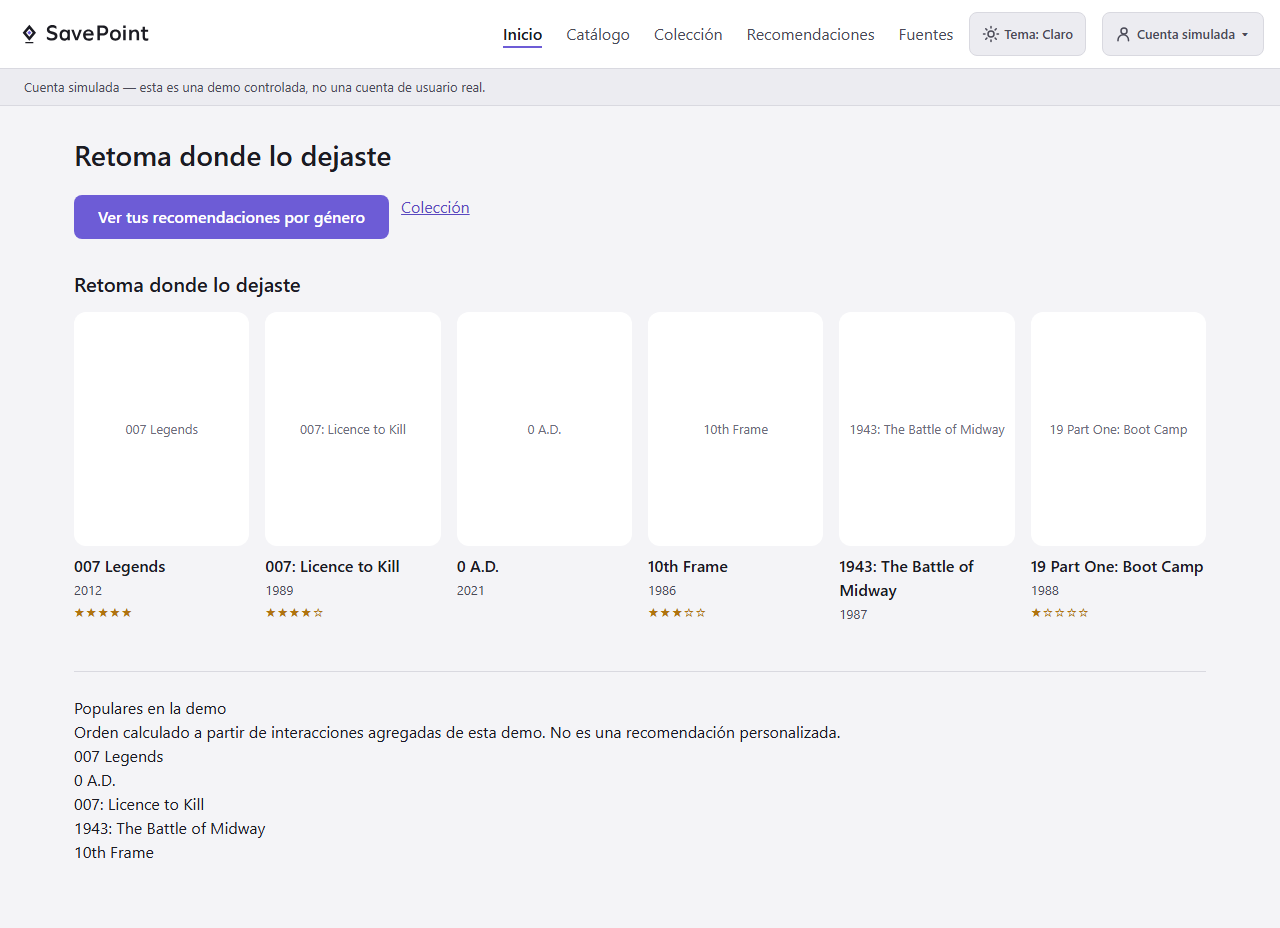
\includegraphics[width=0.82\textwidth]{figures/captura-home-claro}
\caption{Portada de SavePoint en tema claro. Fuente: captura del proyecto.}\label{fig:inicio}
\end{figure}

\begin{figure}[H]
\centering
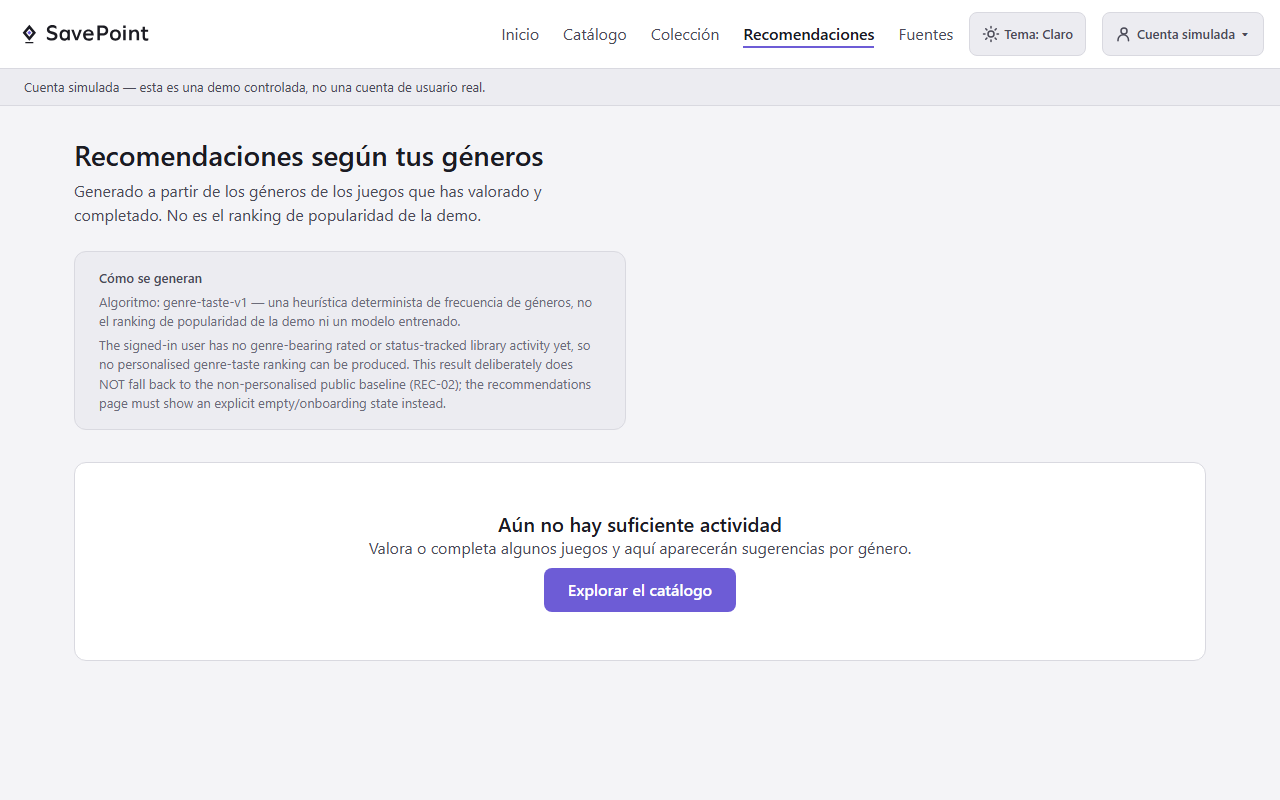
\includegraphics[width=0.82\textwidth]{figures/captura-recomendaciones}
\caption{Vista de recomendaciones de la aplicación. Fuente: captura del proyecto.}\label{fig:recomendaciones-ui}
\end{figure}

La verificación combina pruebas de backend contra PostgreSQL real (unitarias e integración en
una única suite \texttt{pytest}, sin separarlas en conteos independientes), pruebas de
frontend con Vitest y un recorrido de navegador con Playwright que integra los casos de
accesibilidad mediante \texttt{axe}, sin un conteo aislado solo de accesibilidad. El cierre de
evidencia de la Fase 7, ejecutado el 14 de septiembre de 2026 y registrado en
\texttt{docs/verification/phase-07-launch-gate.md} y en \texttt{07-VERIFICATION.md}, deja como
última regresión completa 736 pruebas de backend, 70 de frontend y 56 de navegador, las tres
en verde y sin omitidas. Las evidencias de seguridad, migraciones, privacidad, importación y
exportación se citan desde \texttt{docs/verification/}.

\section{Despliegue}\label{cap:despliegue}

La restricción de partida del despliegue público es la misma que ya fijó su diseño: coste
cero, sin introducir ninguna tarjeta de pago ni habilitar ningún recurso de facturación. La
Tabla~\ref{tab:topologia} recoge el contrato de cada superficie.

\begin{table}[H]
\centering
\begin{tabularx}{\textwidth}{ | Y | Y | Y | }
    \hline
    \textbf{Superficie} & \textbf{Servicio} & \textbf{Contrato} \\
    \hline
    Interfaz de navegador & Vercel Hobby & Construye el frontend Next.js; reenvía del lado del servidor las rutas de la API y de salud hacia Render. \\
    \hline
    API & Render Free & Construye la imagen de la API con el catálogo local congelado y expone la ruta de salud. \\
    \hline
    Base de datos & Neon Free & Proyecto \texttt{autumn-breeze-06234770}, rama \texttt{production}; suministra PostgreSQL a Render. \\
    \hline
\end{tabularx}
\caption{Topología pública aprobada, de coste cero.}
\label{tab:topologia}
\end{table}

El navegador solo ve el origen HTTPS de Vercel. La variable que apunta al backend existe
únicamente en el entorno de servidor de Next.js, de modo que las cookies de sesión y de
protección contra falsificación de petición en sitios cruzados que emite Django siguen siendo
del mismo origen. En Render, la cadena de arranque encadena migración, importación del
catálogo, creación de cuentas simuladas y semilla; solo entonces cede el control al servidor
\texttt{gunicorn}, con cada paso idempotente y protegido con un bloqueo consultivo, de modo que
un paso fallido detiene el arranque, tal como resume la Figura~\ref{fig:despliegue-flujo}.

\begin{figure}[H]
    \centering
    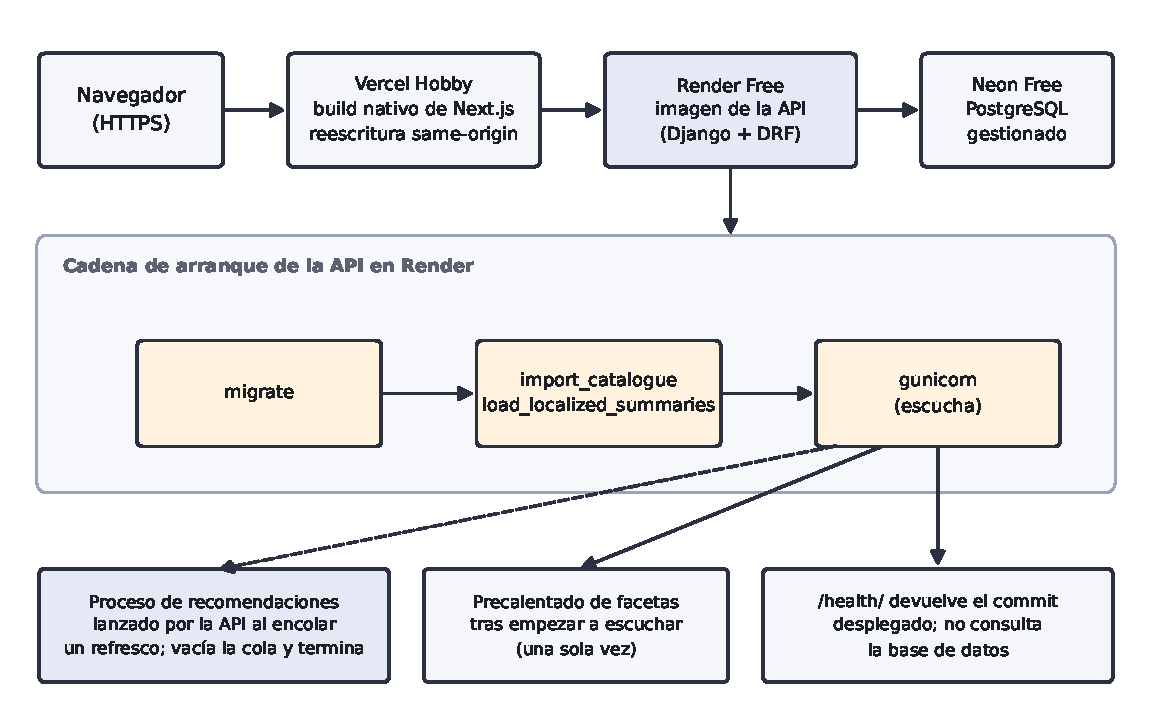
\includegraphics[width=0.92\textwidth]{figures/despliegue-flujo.pdf}
    \caption{Topología de despliegue público y cadena de arranque en Render.}
    \label{fig:despliegue-flujo}
\end{figure}

Docker Compose sigue siendo el entorno reproducible canónico, con los tres componentes de
aplicación (base de datos, API y frontend) y los \textit{workers} de recomendación construidos
desde sus ficheros de Docker. La equivalencia con el
despliegue público es funcional, de versiones, de commit y de datos, no de imagen byte a
byte: el frontend público lo construye Vercel de forma nativa y no ejecuta la imagen de Docker
del frontend, una diferencia de despliegue documentada, no una divergencia de comportamiento.
Si cualquier servicio gratuito duerme, cambia sus términos o desaparece, el entorno local sigue
disponible sin conexión. Los límites conocidos del nivel gratuito se declaran de forma
explícita: el servicio de la API en Render duerme tras quince minutos sin tráfico, de modo que
un visitante puede encontrar un arranque en frío de cerca de un minuto; las cuotas mensuales de
los tres proveedores pueden suspender un servicio, y el nivel gratuito no promete copias de
seguridad ni restauración.

La demostración pública está en vivo desde el 5 de septiembre de 2026, con la prueba de humo en
verde contra la revisión desplegada. En ese despliegue sirve la interfaz anterior al rediseño
contra el corpus curado de ciento cincuenta juegos de Wikidata: el rediseño de la interfaz y el
catálogo a escala real no están en el despliegue público, sino integrados en la rama principal
y ejecutados en el entorno local de Docker Compose. El frontend rediseñado llegó a construirse
en Vercel, pero la base de datos desplegada todavía contiene solo el corpus curado, de modo que
la vista de catálogo da error contra ese despliegue; se revisó esta situación y se decidió
dejar el despliegue público actual como está por ahora, con la demostración ante el tribunal
ejecutándose desde el entorno local reproducible. Conectar el despliegue a datos reales de
internet (cargar el catálogo de IGDB en una base de datos desplegada, aplicar las migraciones
nuevas y ajustar la configuración de hosts y de proxies) queda pospuesto al final del proyecto:
es una decisión registrada, no un defecto pendiente.

Este capítulo ha descrito el producto completo, de los requisitos al despliegue. El
Capítulo~\ref{cap:nucleo-investigacion} recorre el otro núcleo del trabajo, los algoritmos de
recomendación que se construyen sobre esta misma plataforma, y el Capítulo~\ref{cap:conclusiones}
cierra la memoria con el grado de cumplimiento de los objetivos y las líneas de continuación.


    \part{Cierre}\label{part:construccion}
    \chapter{Conclusiones y continuidad}\label{cap:conclusiones}

SavePoint entrega una plataforma funcional y un banco de pruebas de recomendación con un énfasis explícito en procedencia, trazabilidad y reproducibilidad. La contribución principal no es una única lista de juegos, sino el mecanismo que permite relacionar un ranking con sus señales, datos, parámetros, candidatas, métricas y artefactos. El autor diseñó y aplicó una metodología de ingeniería asistida por agentes, gobernada mediante GSD, organizada conceptualmente con Obsidian y validada mediante pruebas, revisiones y evidencias versionadas.

La publicación v15 muestra diferencias numéricas entre baselines, contenido, colaborativo e híbrido bajo sus condiciones fijadas. La evidencia no permite extrapolar esas cifras a usuarios reales ni convertir un único run de 79 usuarios sintéticos evaluables en superioridad científica general. Esa limitación es parte del resultado: delimita con precisión qué se ha demostrado y qué debe comprobarse después.

Las líneas de continuación son repetir el protocolo con nuevas semillas y cohortes, incorporar evaluación con usuarios y consentimiento, estudiar sensibilidad de pesos e hiperparámetros, completar las capturas y diagramas verificables, y consolidar el registro de esfuerzo y pruebas para la defensa. Cualquier extensión deberá crear un protocolo y artefacto nuevos, sin alterar retrospectivamente la evidencia v15.


    % Registro técnico detallado de las fases de ingeniería.
    \appendix
    \part{Apéndices técnicos y registro de ingeniería}\label{part:apendices}
    \chapter{Planificación y metodología de trabajo}\label{cap:metodologia}

Este capítulo describe cómo se ha organizado el trabajo. Empieza por los objetivos de
gestión y por el método de desarrollo iterativo. Después detalla la metodología de ingeniería
gobernada mediante GSD, que el planteamiento del trabajo pide tratar como una aportación
observable y no como una nota al margen. Termina con la estimación de esfuerzo, los riesgos,
las lecciones de ingeniería más relevantes y las convenciones de commits y de idioma.

\section{Objetivos de gestión}\label{sec:met-objetivos-gestion}

La gestión del proyecto persigue cuatro objetivos. El primero es entregar valor de forma
incremental, con cada incremento vertical utilizable y verificado, en lugar de una
integración final de riesgo. El segundo es que toda afirmación de la memoria tenga respaldo:
una decisión registrada, una verificación independiente o una firma de aceptación. El tercero es
mantener el alcance bajo control a lo largo de sucesivos incrementos, sin que el trabajo de
uno contamine el de otro. El cuarto es que el proceso de ingeniería quede documentado con el
mismo rigor que el producto, de modo que un tercero pueda reconstruir no solo el sistema,
sino la secuencia de decisiones que lo produjo.

\section{Método de desarrollo iterativo}\label{sec:met-fases}

El ciclo de vida del proyecto se gobernó mediante el método \textit{Get Stuff Done}
(GSD)~\cite{gsd}, un sistema de desarrollo dirigido por especificación pensado para agentes de
código, versionado en el propio repositorio. GSD descompone el trabajo en incrementos
verticales y somete cada uno a un ciclo ordenado de cuatro pasos que la
Figura~\ref{fig:ciclo-gsd} resume: discutir, planificar, ejecutar y verificar. Cada paso
produce un artefacto escrito que actúa como fuente de verdad del siguiente. Lo que sobrevive
a los límites de sesión es la especificación escrita, no el historial de la conversación con
el agente.

\begin{figure}[H]
    \centering
    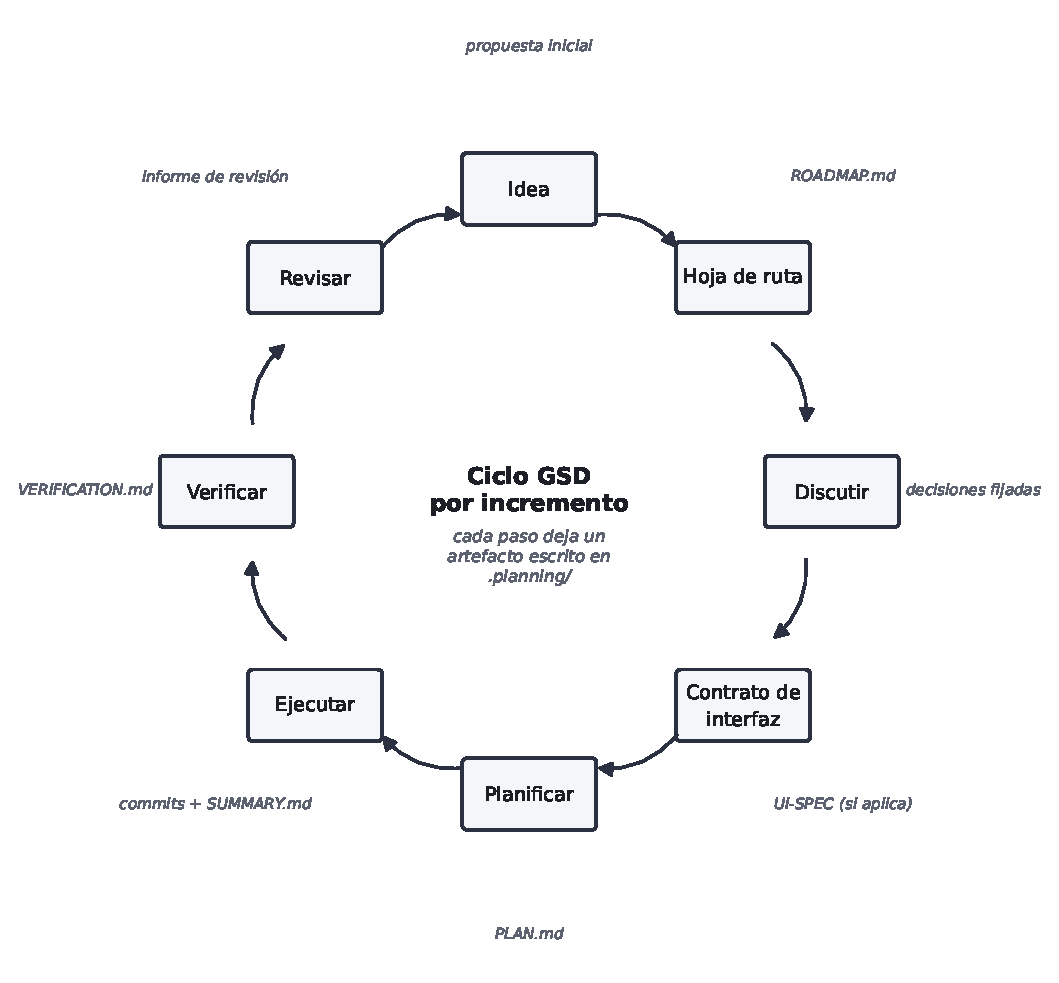
\includegraphics[width=0.72\textwidth]{figures/ciclo-gsd.pdf}
    \caption{Ciclo de un incremento en el método GSD y los artefactos que produce cada paso.}
    \label{fig:ciclo-gsd}
\end{figure}

En la práctica, cada incremento se abre con una discusión que fija por escrito sus decisiones
y supuestos. Si tiene interfaz, se establece además un contrato de diseño con sus componentes
y estados. A continuación se investiga y se redacta el plan, que lo descompone en tareas
atómicas con criterios de aceptación y se comprueba antes de tocar código. La ejecución
implementa ese plan, confirma los cambios en el control de versiones y registra en un resumen
lo realmente hecho y las desviaciones. Por último, la verificación comprueba, de forma
independiente, que el objetivo se ha alcanzado. Una revisión de código somete después los
cambios a un análisis de seguridad, rendimiento y corrección con un contexto distinto del que
los escribió. Cada incremento termina con una firma de aceptación del proyecto.

Las órdenes de este flujo se usaron de verdad durante el proyecto: \texttt{discuss-phase},
\texttt{ui-phase}, \texttt{plan-phase}, \texttt{execute-phase}, \texttt{verify-work},
\texttt{code-review}, además de \texttt{pause-work} y \texttt{resume-work} para suspender y
retomar el trabajo entre sesiones sin perder el hilo.

\section{Planificación viva: el árbol \texttt{.planning/}}\label{sec:met-planning}

GSD sustituye los documentos de planificación estáticos por un árbol de ficheros en formato
Markdown, versionados, que evolucionan con el proyecto. En \texttt{.planning/} conviven la
definición del producto (\texttt{PROJECT.md}), los requisitos operativos
(\texttt{REQUIREMENTS.md}), la hoja de ruta (\texttt{ROADMAP.md}) y una instantánea
del estado actual (\texttt{STATE.md}) que cualquier agente o persona lee antes de actuar.
Cada incremento se descompone en \texttt{.planning/phases/} en pares de plan y resumen: el
plan fija el alcance y los criterios de aceptación antes de implementar, mientras que el
resumen registra lo ejecutado, las desviaciones y las evidencias al cerrar. Junto a ellos
viven los documentos de contexto, investigación, contrato de interfaz, verificación e ítems
diferidos de cada incremento. Junto a este árbol normativo, el proyecto mantiene en
\texttt{ideas-vault/} un vault de Obsidian que enlaza los mismos conceptos entre sí de forma
navegable; el Capítulo~\ref{cap:gestion} lo describe con su propio grafo.

La Tabla~\ref{tab:planning-arbol} enumera los artefactos principales del árbol y su función.

\begin{table}[H]
\centering
\begin{tabularx}{\textwidth}{ | Y | Y | }
    \hline
    \textbf{Artefacto} & \textbf{Función} \\
    \hline
    \texttt{PROJECT.md} & Definición del producto, valor central, requisitos activos y fuera de alcance. \\
    \hline
    \texttt{REQUIREMENTS.md} & Catálogo de requisitos con identificador estable y matriz de trazabilidad a evidencia. \\
    \hline
    \texttt{ROADMAP.md} & Incrementos, objetivos, criterios de éxito y progreso. \\
    \hline
    \texttt{STATE.md} & Estado actual, posición, decisiones acumuladas y continuidad de sesión. \\
    \hline
    \path{phases/<incremento>/<plan>-PLAN.md} & Alcance y criterios de aceptación de un plan, antes de implementar. \\
    \hline
    \path{phases/<incremento>/<plan>-SUMMARY.md} & Lo realmente ejecutado, desviaciones y evidencias, al cerrar el plan. \\
    \hline
    \path{phases/<incremento>/<incremento>-VERIFICATION.md} & Verificación independiente del objetivo del incremento. \\
    \hline
    \path{phases/<incremento>/deferred-items.md} & Hallazgos fuera de alcance, enrutados a trabajo posterior. \\
    \hline
\end{tabularx}
\caption{Artefactos principales del árbol \texttt{.planning/}.}
\label{tab:planning-arbol}
\end{table}

\section{Trazabilidad de tareas, requisitos y evidencias}\label{sec:met-trazabilidad}

La trazabilidad se apoya en tres mecanismos. El primero es la matriz de
\texttt{REQUIREMENTS.md}, que registra el estado de cada requisito y la evidencia que lo
cierra, de modo que cualquier requisito se puede seguir hasta el trabajo que lo entrega y
hasta la prueba que lo respalda. El segundo es la correspondencia entre planes e incidencias:
cada plan tiene un issue de GitHub asociado, que se cierra a medida que la ejecución avanza,
lo que enlaza el seguimiento externo con el árbol de planificación. El tercero es el registro
de agentes descrito en la Sección~\ref{sec:met-ledger}, que ata cada artefacto a la acción
que lo produjo mediante un hash de contenido. Entre los tres, una decisión de la memoria se
puede recorrer hacia atrás hasta su plan, su requisito y su discusión; hacia delante llega
hasta la prueba y la firma que la verifican.

\section{Planificación de la Fase 2: del producto al laboratorio}\label{sec:met-fase2}

La Fase 2 se planificó como el puente entre la demostración de producto y la investigación
reproducible. Su objetivo no era añadir una pantalla aislada, sino fijar las condiciones que
permiten afirmar algo sobre un recomendador: qué obras entran en el corpus, qué significan
las valoraciones, qué usuarios se simulan, cómo se construyen los candidatos y con qué
métricas se comparan las listas. Las decisiones metodológicas se tomaron antes de cualquier
ejecución de laboratorio y se conservaron en el directorio de planes de la fase.

La planificación se dividió en seis olas. Las dos primeras cerraron la frontera del corpus,
los ratings y el protocolo. La tercera reunió la búsqueda, la API de catálogo, los usuarios
sintéticos y las primeras primitivas del recomendador. La cuarta reservó la interfaz de
filtros y las variantes de contenido; la quinta, la ficha y la ejecución comparativa; y la
sexta, la página final de recomendaciones. De esos planes, 02-01, 02-02, 02-03, 02-05, 02-07, 02-08, 02-09 y 02-10 quedaron cerrados y
verificados; el resto se fue incorporando en incrementos posteriores, según recoge
\texttt{ROADMAP.md}.

El orden no es accidental. El corpus y el snapshot preceden al protocolo; el protocolo
precede a la generación de usuarios y a la implementación de variantes; y solo entonces se
puede ejecutar una comparación con garantías de que todos los algoritmos han recibido la
misma partición y el mismo conjunto de candidatos. Una tarea completada ha superado las
verificaciones de su contrato, pero no demuestra una superioridad algorítmica.

\subsection{Decisiones previas a las pruebas de laboratorio}

Las decisiones que bloquean una comparación posterior quedaron congeladas en
\texttt{docs/methodology/protocol.json} y en
\texttt{docs/methodology/evaluation-protocol.md}. El corpus se define mediante una vista
versionada de obras principales con fecha, género y al menos una plataforma de la lista de
39 plataformas. La ausencia de rating no excluye una obra. La vista es reversible y conserva
el catálogo fuente para que una nueva decisión pueda producir otra versión sin reescribir la
anterior.

Las valoraciones de investigación se almacenan en
\texttt{CorpusRatingSnapshot}. El modelo es insert-only por pareja de obra, fuente y versión
de corpus. IGDB actúa como fuente primaria y RAWG como contraste acotado. El número mostrado
en la ficha puede combinar información externa y valoraciones locales, pero esa mezcla
pertenece al producto y no se utiliza como entrada mutable del laboratorio.

La relevancia quedó fijada como una entrada de biblioteca con estado completado y una
valoración de al menos siete medias estrellas
(\texttt{rating\_half\_steps >= 7}). Para cada usuario se retiene una obra mediante
\textit{leave-one-out}, con semilla 20260907; después se devuelve al conjunto de candidatos. Este
conjunto es el corpus gobernado menos cualquier obra presente en la biblioteca, más la obra
retenida. De este modo, todos los algoritmos predicen exactamente el mismo caso y no
recomiendan obras ya conocidas.

La población sintética generada en la Wave 3 combina ocho escenarios: monogénero severo,
monogénero generoso, omnívoro medio, completista de saga, explorador de novedades,
coleccionista de pendientes, jugador ocasional cold-start y veterano de biblioteca grande.
Cada arquetipo varía el número de géneros preferidos, el tamaño de la biblioteca, la
generosidad al puntuar y la mezcla de estados. Sus usuarios se identifican con el marcador
\texttt{synthetic-eval-user} y una semilla por arquetipo, de modo que no contaminan el
baseline de popularidad de la aplicación ni se presentan como actividad real.

El protocolo utiliza \texttt{precision@k}, \texttt{recall@k}, \texttt{nDCG@k} y
\texttt{MAP@k}, para $k\in\{5,10,20\}$; fija \texttt{nDCG@10} como métrica titular. La
rejilla de ajuste contiene 18 configuraciones, se selecciona en validación y el conjunto de
prueba solo se puede consumir una vez. El protocolo declara explícitamente que la población
es simulada: la ejecución de referencia produjo 200 usuarios y una cohorte independiente
de 25 perfiles cold-start, con entre uno y tres juegos por perfil. Sus distribuciones de
biblioteca, ratings y estados se conservan en el informe de verificación del repositorio.

\subsection{Ratificaciones, incidencias y límites}

Se ratificó la lista de plataformas, la incorporación acotada de RAWG, el protocolo
propuesto y la implementación del primer modelo de features con Python puro. RAWG se ejecutó
en 18 lotes de 500 peticiones para limitar el coste de un reinicio y mantener la idempotencia.
Se emparejaron 8.575 de 10.000 obras, pero la cobertura combinada siguió siendo 27.014 de
193.885 obras gobernadas (13,9330\%), porque la selección estaba ordenada por
\texttt{rating\_count} de IGDB. RAWG aporta, por tanto, contraste de fuente y no cobertura
adicional en ese corte.

El importador actual no tiene cobertura suficiente de franquicias ni desarrolladores. El
vector de contenido los excluye mediante un gate de cobertura en lugar de imputarlos. La
mezcla de rating mostrada en la ficha también quedó señalada para confirmación del proyecto y
no debe confundirse con el término de rating del laboratorio, que procede del snapshot
inmutable.

\section{Agentes de GSD y skills}\label{sec:met-agentes}

El proyecto se desarrolló con asistencia sistemática de los agentes especializados que define
GSD. Conviene delimitar desde el principio el reparto de responsabilidades, que la
Sección~\ref{sec:met-encuadre} retoma: los agentes ejecutan, mientras que la definición del
alcance, los criterios de aceptación, la revisión de cada entrega y la decisión final son
del proyecto. El uso de agentes se describe aquí como una metodología de trabajo que se
diseñó, dirigió y evaluó, no como una coautoría.

\subsection{Subagentes, aislamiento y skills}\label{sec:met-subagentes}

El obstáculo práctico del trabajo prolongado con un agente es la degradación del contexto: la
ventana de contexto se satura de historial y la calidad de las respuestas decae hasta
contradecir decisiones anteriores~\cite{anthropic-context}. La respuesta adoptada combina tres
mecanismos. El primero es el aislamiento del contexto: el trabajo se descompone en tareas
atómicas, cada una ejecutada por una instancia nueva del agente con la ventana limpia, y la
información viaja entre tareas a través de los ficheros de memoria persistentes del árbol
\texttt{.planning/} en lugar de a través del historial de la conversación, de modo que una
interrupción, un límite de sesión o un cambio de día no hacen perder el hilo: la sesión
siguiente relee el estado y continúa. El segundo es la especialización de esas instancias en
papeles distintos, resumidos en la Tabla~\ref{tab:subagentes}: quien planifica, quien implementa
y quien verifica son instancias independientes, de modo que la verificación no hereda la
confianza del código recién escrito, y esta división reproduce con agentes la separación entre
desarrollo y revisión propia de un equipo humano.

\begin{table}[H]
\centering
\begin{tabularx}{\textwidth}{ | Y | Y | }
    \hline
    \textbf{Rol} & \textbf{Responsabilidad y límite} \\
    \hline
    \texttt{gsd-phase-researcher} & Recopila y sintetiza evidencia para planificar un incremento. Propone; etiqueta fuente, evidencia o supuesto. \\
    \hline
    \texttt{gsd-ui-researcher} / \texttt{gsd-ui-checker} & Convierten los requisitos en un contrato de diseño y lo validan. La comprobación automática de accesibilidad no sustituye la revisión humana. \\
    \hline
    \texttt{gsd-planner} & Divide el alcance en tareas verificables. Propone secuencia y gates; no declara terminado el producto. \\
    \hline
    \texttt{gsd-executor} & Implementa, prueba y registra correcciones en una copia de trabajo aislada, con commits atómicos. No se presenta como verificación independiente. \\
    \hline
    \texttt{gsd-verifier} & Verifica el objetivo del incremento de forma independiente y escribe el informe de verificación. \\
    \hline
    \texttt{gsd-code-reviewer} & Revisa todo el repositorio en busca de defectos con un contexto propio, distinto del de la implementación. \\
    \hline
\end{tabularx}
\caption{Subagentes empleados y su responsabilidad.}
\label{tab:subagentes}
\end{table}

El tercer mecanismo refuerza el aislamiento a nivel de sistema de ficheros: cada ejecución de
un plan se realiza sobre una copia de trabajo aislada de Git, un \textit{worktree}, con su
propia rama; el ciclo es crear el worktree, ejecutar el plan en él con commits atómicos,
integrarlo en la rama principal con una fusión sin avance rápido y limpiar la copia, de modo que
un plan a medias nunca deja el árbol principal en un estado inconsistente y la integración de
cada plan queda registrada como un punto único en el historial. Junto a estos tres mecanismos,
el repositorio versiona además \textit{skills}, conjuntos de instrucciones reutilizables que un
agente invoca durante el desarrollo: al vivir junto al código, el entorno de trabajo del agente
forma parte del entregable, y un tercero que clone el repositorio obtiene tanto el sistema como
las instrucciones con las que se construyó.

\subsection{Contrato de contexto y memoria persistente}\label{sec:met-contrato-contexto}

El repositorio define un contrato de contexto común que toda herramienta lee al empezar cada
sesión. Los ficheros \texttt{AGENTS.md}, \texttt{CLAUDE.md} y
\texttt{.github/copilot-instructions.md} reúnen la arquitectura, las convenciones y el
protocolo obligatorio para Claude, Codex, GitHub Copilot u otra herramienta. El documento
canónico de convenciones es \texttt{CONVENTIONS.md}, que prevalece sobre cualquier otra
instrucción en conflicto. Un ejemplo de regla transversal es la convención de idioma, vigente
desde el 6 de septiembre de 2026: la documentación de la tesis y la prosa nueva de
planificación se escriben en español, mientras que el código, con sus identificadores,
comentarios, mensajes de commit y nombres de rama, se mantiene en inglés, con las citas legales
textuales conservadas en su idioma original para no perder valor probatorio.

Sobre ese mismo contrato se apoyan los ficheros de memoria del agente, que sobreviven entre
sesiones: cuando un error del agente o una corrección del proyecto tiene valor general, se
destila en una regla que se relee al iniciar cada tarea, de modo que el fallo no se repite. El
proyecto acumuló varias reglas de este tipo a partir de incidencias reales:

\begin{itemize}
    \item La lista de identificadores de Wikidata escrita a mano en el guion de adquisición
    contenía entidades que no eran videojuegos. La regla derivada obliga a verificar en vivo
    cualquier identificador de Wikidata antes de usarlo, sin confiar en la memoria ni en un
    commit anterior.
    \item El primer intento de cargar el catálogo de IGDB junto al corpus de Wikidata abortó
    por una colisión de \textit{slug} de plataforma. La corrección enseñó al importador a
    reconciliar una plataforma existente por \textit{slug}, nombre e inserción dentro de un
    savepoint, en lugar de fallar. El mismo patrón de convivir con estado preexistente
    resolvió más tarde el arranque de las cuentas simuladas plurales, cuando el comando de
    arranque adoptó la cuenta primaria heredada bajo una clave de anclaje en lugar de abortar
    por colisión.
    \item Los enganches de GSD fallaban en Windows por un problema de shell. Detectarlo y
    corregirlo pronto evitó que el resto del trabajo tropezara con lo mismo.
    \item Sin un montaje enlazado de Docker y sin cargar el módulo de configuración de Django
    dentro del contenedor, toda verificación posterior habría probado una imagen obsoleta o
    habría fallado al arrancar. Corregir ambos al detectarlos evitó que el trabajo siguiente
    chocara con la misma pared.
\end{itemize}

\subsection{El registro de agentes}\label{sec:met-ledger}

El componente más distintivo del proceso es el registro de agentes,
\texttt{docs/methodology/agent-ledger.jsonl}, un fichero de solo anexado con un objeto por
línea. Cada entrada lleva una marca de tiempo, un tipo, el actor, el objetivo, las entradas y
salidas referenciadas por ruta relativa y hash SHA-256, las herramientas empleadas sin sus
secretos, el resultado y las limitaciones declaradas. El tipo es uno de tres:
\texttt{proposal} para una propuesta de agente, \texttt{automated-check} para una
comprobación determinista y \texttt{author-decision} para una decisión humana, que siempre
identifica al actor como persona. El registro contiene veinticinco entradas. El gate
\texttt{scripts/check-evidence.ps1} valida su esquema, sus tipos, sus actores, sus rutas, sus
hashes y su cobertura, probando primero con entradas inválidas antes de dar por buena una
ejecución limpia.

El registro es una convención auditable, no un almacén criptográficamente inmutable: Git
conserva las revisiones y el gate detecta corrupción de referencias en el estado actual, pero
un actor con permiso de escritura podría reescribir el historial. Para la evidencia final se
firma o etiqueta el commit correspondiente. El registro es honesto sobre sus propios huecos:
donde un artefacto histórico resultó irrecuperable, la entrada lo declara en sus campos de
entradas no verificables y de limitaciones en lugar de ocultarlo o falsearlo. También registra
que el proyecto usó más de un entorno de agente, la familia \texttt{gpt-5} sobre Codex en el
trabajo inicial y Claude en el trabajo posterior, con la advertencia de que un nombre de
modelo no basta para reproducir una salida probabilística: la evidencia reproducible son los
artefactos versionados, los hashes, los comandos y las decisiones humanas.

\subsection{Beneficios, límites y encuadre}\label{sec:met-encuadre}

El enfoque produjo beneficios concretos y observables en el proyecto, junto con límites que
conviene declarar con la misma franqueza. El alcance se mantuvo bajo control a lo largo de
sucesivos incrementos, sin que el trabajo de uno se filtrara en otro, y cada cambio quedó
trazado hasta su plan, su requisito y su evidencia. Las revisiones de código con contexto
independiente encontraron dieciséis hallazgos reales, descritos en el
Capítulo~\ref{cap:pruebas}, que se corrigieron por completo, incluidos defectos de seguridad en
trabajo ya dado por bueno. El trabajo se pudo reanudar sin pérdida de hilo tras interrupciones
y límites de sesión, porque el estado vivía en ficheros y no en una conversación, y el propio
proceso de ingeniería quedó reproducible, no solo el producto: un tercero puede clonar el
repositorio y reconstruir la historia de decisiones a partir del árbol de planificación, los
registros de decisión, el registro de agentes y los gates de evidencia.

El enfoque depende, sin embargo, de la calidad de la especificación escrita: un plan ambiguo
produce una ejecución ambigua. Mantener la disciplina de planificación, verificación y registro
tiene un coste de tiempo notable para un TFG individual, y los agentes cometieron errores que
hubo que detectar y corregir, algunos de ellos recogidos en la
Sección~\ref{sec:met-contrato-contexto}. Un agente no es un evaluador independiente de su
propia propuesta, del mismo modo que un hash prueba identidad de bytes, no veracidad ni calidad;
por eso el enfoque no sustituye el juicio del proyecto sobre arquitectura, alcance y aceptación,
sino que lo enmarca. Existe un informe de uso de herramientas de asistencia, independiente y
posterior, que cubre la transparencia de su empleo; esta memoria ni lo suple ni lo contradice.

\section{Registro de incidencias y decisiones}\label{sec:met-incidencias}

Además del registro de agentes, el proyecto conserva dos registros de decisión. Los ítems
diferidos, en \texttt{deferred-items.md}, recogen los hallazgos fuera de alcance descubiertos
durante la ejecución, con su motivo y su destino. Los registros de decisión de arquitectura,
en \texttt{docs/adr/}, documentan cada decisión material con su contexto, sus alternativas,
su decisión, su evidencia, sus consecuencias y su reversibilidad. El
Capítulo~\ref{cap:diseno} resume los nueve registros de decisión de arquitectura vigentes.

\section{Planificación temporal}\label{sec:met-temporal}

El trabajo se planificó como una sucesión de incrementos verticales, cada uno utilizable y
verificado antes de abordar el siguiente, en lugar de un calendario cerrado de tareas fijado
desde el principio. El desarrollo se organizó en seis iteraciones a lo largo de cuatro meses,
del 2 de junio al 30 de septiembre de 2026, agrupadas alrededor de los hitos de la
Tabla~\ref{tab:hitos}.

\begin{table}[H]
\centering
\caption{Lista de hitos del trabajo.}\label{tab:hitos}
\begin{tabularx}{\textwidth}{ | Y | Y | }
    \hline
    \textbf{Hito} & \textbf{Fecha} \\
    \hline
    H0 — Aprobación de la propuesta y arranque del repositorio & 02/06/2026 \\
    \hline
    H1 — Demostración pública de tres días en producción (Fase 1) & 12/06/2026 \\
    \hline
    H2 — Catálogo a escala real e interfaz rediseñada (Fase 01.1) & 03/07/2026 \\
    \hline
    H3 — Contrato de evaluación offline congelado (Fase 2) & 24/07/2026 \\
    \hline
    H4 — Recomendadores de contenido, colaborativo e híbrido implementados & 14/08/2026 \\
    \hline
    H5 — Publicación de resultados v15 con significación estadística & 12/09/2026 \\
    \hline
    H6 — Flujos de colección, descubrimiento público y endurecimiento cerrados & 14/09/2026 \\
    \hline
    H7 — Memoria del TFG completa, lista para defensa & 30/09/2026 \\
    \hline
\end{tabularx}
\end{table}

La \textbf{Iteración 1} (2 al 14 de junio) cubrió el estudio previo: revisión de productos de
referencia, comparación de fuentes de datos de videojuegos y sus licencias, y las primeras
decisiones de arquitectura (ADR-001 y ADR-002); cerró con un entorno de desarrollo
reproducible en Docker Compose. La \textbf{Iteración 2} (15 de junio al 3 de julio) entregó el
primer incremento de producto bajo una restricción explícita de tres días para una
demostración pública visible, con un catálogo reducido, una cuenta y la recomendación por
popularidad; a continuación amplió el catálogo a escala real e incorporó el rediseño de la
interfaz. La \textbf{Iteración 3} (4 al 24 de julio) congeló el contrato de evaluación offline:
corpus, población sintética, métricas y protocolo, antes de escribir ningún algoritmo de
recomendación avanzado. La \textbf{Iteración 4} (25 de julio al 14 de agosto) implementó las
tres familias de recomendación (contenido, colaborativo e híbrido) y sus dieciséis variantes.
La \textbf{Iteración 5} (15 de agosto al 13 de septiembre) cerró los flujos completos de
colección y portabilidad, el descubrimiento público, el endurecimiento de seguridad y el panel
de investigación; ejecutó también la publicación final de resultados (v15) descrita en la
Sección~\ref{cap:experimentos}. La \textbf{Iteración 6} (14 al 30 de septiembre) se dedicó por
completo a la redacción, revisión y cierre de esta memoria.

Cada incremento se cerró con una verificación de objetivo independiente y una firma de
aceptación del proyecto, de modo que ninguna iteración empezó sobre una anterior sin cerrar; la
Sección~\ref{sec:met-fase2} y la Sección~\ref{cap:experimentos} detallan cómo esa disciplina
se aplicó dentro del propio núcleo de investigación.

\section{Estimación de esfuerzo y presupuesto}\label{sec:met-presupuesto}

El proyecto no llevó un registro de horas minuto a minuto por tarea, de modo que la estimación
de esfuerzo que sigue se reconstruye a partir de la duración de cada iteración y de la carga de
trabajo declarada de un estudiante que compagina el TFG con otras obligaciones académicas,
en torno a veinticinco horas semanales durante las diecisiete semanas del proyecto. Tomando
como unidad el bloque de trabajo, no el incremento, la Tabla~\ref{tab:presupuesto-horas}
reparte esas horas entre las grandes áreas del trabajo.

\begin{table}[H]
\centering
\caption{Estimación de horas por bloque de trabajo.}\label{tab:presupuesto-horas}
\begin{tabularx}{\textwidth}{ | Y | Z | }
    \hline
    \textbf{Bloque} & \textbf{Horas estimadas} \\
    \hline
    Análisis, requisitos y diseño & 60 \\
    \hline
    Infraestructura reproducible y despliegue & 35 \\
    \hline
    Implementación de producto (backend y frontend) & 120 \\
    \hline
    Adquisición y gobierno de datos & 40 \\
    \hline
    Algoritmos de recomendación y protocolo de evaluación & 90 \\
    \hline
    Pruebas, verificación y revisión & 45 \\
    \hline
    Redacción de la memoria & 50 \\
    \hline
    \textbf{Total} & \textbf{440} \\
    \hline
\end{tabularx}
\end{table}

El coste directo se calcula sobre esas 440 horas con una tarifa de referencia de un perfil
junior de ingeniería del software en España, 14,00\,€/hora, una cota conservadora frente al
coste real de contratación de un perfil equivalente. El coste material recoge la amortización
proporcional del equipo personal empleado (un portátil de gama media, con una vida útil
estimada de cuatro años, del que este trabajo consume cuatro meses); no se incluye ningún coste
de infraestructura en la nube, porque la topología de despliegue público se diseñó
explícitamente de coste cero (ADR-005, Sección~\ref{cap:despliegue}). El coste indirecto
recoge la cuota proporcional de cuatro meses de electricidad y conexión a internet atribuible
al proyecto. La Tabla~\ref{tab:presupuesto} resume el presupuesto total.

\begin{table}[H]
\centering
\begin{tabularx}{\textwidth}{ | Y | Z | }
    \hline
    \textbf{Concepto} & \textbf{Coste (\euro{})} \\
    \hline
    Coste directo (440\,h a 14,00\,€/h) & 6.160,00 \\
    \hline
    Coste material (amortización de equipo, 4 meses) & 75,00 \\
    \hline
    Costes indirectos (electricidad y conexión, 4 meses) & 180,00 \\
    \hline
    \textbf{Presupuesto total} & \textbf{6.415,00} \\
    \hline
\end{tabularx}
\caption{Estimación de esfuerzo y presupuesto del proyecto.}
\label{tab:presupuesto}
\end{table}

Estas cifras son una estimación reconstruida a posteriori, no una medición registrada durante
el desarrollo; así debe entenderse cualquier comparación futura entre coste estimado y coste
real.

\section{Riesgos y mitigaciones}\label{sec:met-riesgos}

La Tabla~\ref{tab:riesgos} recoge los riesgos que se identificaron y cómo se mitigaron o se
mantienen bajo vigilancia.

\begin{table}[H]
\centering
\begin{tabularx}{\textwidth}{ | Y | Y | }
    \hline
    \textbf{Riesgo} & \textbf{Mitigación} \\
    \hline
    Restricción de tres días del primer incremento público & Alcance de demostración deliberadamente estrecho: catálogo pequeño, una cuenta y recomendación por popularidad. \\
    \hline
    Términos legales de las fuentes de datos & Confirmación caso por caso: corpus de Wikidata bajo dominio público, términos de IGDB registrados textualmente y reconciliados en un registro de decisión. \\
    \hline
    Volumen de IGDB en una importación larga & Importador reanudable por cursor de identificador, con checkpoint tras cada lote y resistencia probada a una interrupción. \\
    \hline
    Portadas por enlace directo a un tercero & Ventana de retención de treinta días asumida; ausencia o fallo de una portada cae a un marcador propio. \\
    \hline
    El protocolo de evaluación debe congelarse antes de comparar recomendadores & El heurístico de géneros del sistema se declaró explícitamente fuera de esa comparación desde el principio; la comparación en sí se congeló y se ejecutó más tarde, como recoge la Parte~\ref{part:nucleo-investigacion}. \\
    \hline
    Errores del agente en trabajo dado por bueno & Verificación de objetivos independiente y revisión de código de todo el repositorio con contexto propio. \\
    \hline
    Despliegue no conectado a datos reales & Decisión registrada del proyecto de posponer esa conexión al final del proyecto; el entorno local reproducible es la vía de demostración. \\
    \hline
\end{tabularx}
\caption{Riesgos identificados y sus mitigaciones.}
\label{tab:riesgos}
\end{table}

\section{Lecciones de ingeniería}\label{sec:met-desviaciones}

El trabajo dejó varias lecciones de ingeniería que conviene recoger. La primera surgió al
planificar el crecimiento del catálogo y del sistema de cuentas: la investigación detectó un
conflicto real de alcance con el registro abierto de producción, reservado a una evolución
posterior del producto. Se resolvió con una vía intermedia, un formulario de registro
funcional dentro de la frontera de demostración controlada, sin abrir el registro de
producción sin restricciones. La lección es que un contrato de alcance escrito y revisado
antes de tocar código evita que una funcionalidad aparentemente inocua cruce una frontera de
diseño.

La segunda tiene que ver con el despliegue. La topología pasó de un único proveedor con
predespliegue para las dos imágenes de contenedor a tres servicios gratuitos coordinados, al
chocar la restricción de coste cero con el modelo de un solo proveedor. La decisión y sus
consecuencias quedaron documentadas en un registro de decisión de arquitectura, de modo que
la diferencia entre el despliegue público y el entorno local es una elección deliberada y
no una divergencia de comportamiento.

La tercera es de higiene del propio proceso: un gate de evidencia llegó a estar en rojo en la
rama principal por un problema de fin de línea y por registros de decisión escritos en inglés
antes de fijarse la convención de idioma. Corregirlo en cuanto se detectó evitó que el resto
del trabajo arrastrara un gate poco fiable. Estas incidencias, junto con otras menores,
quedaron registradas en los resúmenes de plan.

\section{Convenciones de commits y de idioma}\label{sec:met-convenciones}

Los mensajes de commit siguen el estilo de \textit{Conventional Commits} y se escriben en
inglés. Toda dependencia directa nueva o cambio de versión exige aprobación humana explícita,
una fila en el registro de legitimidad de dependencias, una fila en el gate correspondiente y
una entrada en el registro de agentes. La convención de idioma descrita en la
Sección~\ref{sec:met-contrato-contexto} separa la documentación, en español, del código, en
inglés, con las citas legales textuales conservadas en su idioma original.

Este capítulo ha descrito el método de trabajo y, con detalle, la metodología asistida por
agentes que lo sostiene. Los capítulos siguientes aplican ese método al análisis, al diseño y
a la construcción del sistema.

    \chapter{Análisis de requisitos}\label{cap:requisitos}

\todo[inline]{Capítulo por redactar en la siguiente iteración.}

    \chapter{Diseño de la solución}\label{cap:diseno}

\todo[inline]{Capítulo por redactar en la siguiente iteración.}

    \chapter{Datos: adquisición, licencias y procedencia}\label{cap:datos}

\todo[inline]{Capítulo por redactar en la siguiente iteración.}

    \chapter{Implementación}\label{cap:implementacion}

\todo[inline]{Capítulo por redactar en la siguiente iteración.}

    \chapter{Pruebas y verificación}\label{cap:pruebas}

Este capítulo describe cómo se comprueba que el sistema hace lo que debe. Presenta la
estrategia de pruebas, los gates de evidencia automáticos, la verificación independiente del
objetivo de cada fase y la revisión de código de todo el repositorio, con sus resultados en
cifras reales tomadas de \texttt{docs/verification/} y de los informes de verificación de las
fases.

\section{Estrategia de pruebas}\label{sec:pru-estrategia}

La estrategia combina cuatro niveles. Las pruebas unitarias y de integración del backend se
ejecutan con \texttt{pytest} contra una instancia real de PostgreSQL 18.6, sin sustituirla
por una base en memoria, porque el sistema depende de restricciones, transacciones y búsqueda
de trigramas que solo se comportan igual sobre el motor real. Las pruebas del frontend usan
\texttt{vitest} para la lógica y los componentes, con una prueba de paridad de claves de
traducción. Las pruebas de extremo a extremo usan Playwright sobre un navegador real, con la
biblioteca \texttt{axe} para las comprobaciones automáticas de accesibilidad frente a las
Pautas de Accesibilidad para el Contenido Web (WCAG) 2.2~\cite{wcag22}. Por último, una
prueba de humo se ejecuta contra la URL pública desplegada y rechaza un despliegue con la
revisión equivocada, tráfico entre orígenes inesperado o peticiones fallidas.

La Tabla~\ref{tab:suites} recoge los resultados de las suites en el momento del cierre de la
Fase 01.1.

\begin{table}[htp]
\centering
\begin{tabular}{ | l | l | l | }
    \hline
    \textbf{Suite} & \textbf{Herramienta} & \textbf{Resultado} \\
    \hline
    Backend & \texttt{pytest} sobre PostgreSQL & 209 pruebas superadas \\
    \hline
    Recomendaciones & \texttt{pytest} & 21 pruebas superadas \\
    \hline
    Frontend, unidad y paridad & \texttt{vitest} & 16 pruebas superadas \\
    \hline
    Construcción del frontend & \texttt{next build} & correcta, sin errores de tipos \\
    \hline
    Extremo a extremo y accesibilidad & Playwright y \texttt{axe} & 41 pruebas superadas; cero incidencias críticas o graves de \texttt{axe} \\
    \hline
\end{tabular}
\caption{Resultados de las suites de pruebas al cierre de la Fase 01.1.}
\label{tab:suites}
\end{table}

Las comprobaciones de \texttt{axe} cubren el catálogo, el detalle, el registro, las
recomendaciones, la página de inicio, el acceso y las fuentes, en escritorio a 1280 por 800
píxeles y en móvil a 375 por 812 píxeles.

\section{Gates de evidencia}\label{sec:pru-gates}

Además de las pruebas, el repositorio tiene gates deterministas que protegen la evidencia. El
gate \texttt{check-secrets.ps1} escanea el árbol de Git, los paquetes de construcción, las
capas de las imágenes y los registros capturados en busca de cadenas con forma de credencial,
y se autoverifica primero contra señuelos sintéticos. El gate \texttt{check-evidence.ps1}
valida el esquema, los tipos, los actores, las rutas, los hashes y la cobertura del registro
de agentes, probando primero con entradas inválidas. El gate \texttt{check-dependencies.ps1}
comprueba que toda dependencia directa está en la lista permitida, fijada a versión exacta,
con su fichero de bloqueo. Los gates \texttt{verify-igdb-*.ps1} comprueban el contenido del
registro de decisión de IGDB, la evidencia del sondeo y la ejecución de importación sobre una
base de datos fresca.

\section{Verificación del objetivo de fase}\label{sec:pru-verificacion-fase}

Cada fase tiene una verificación independiente de su objetivo, realizada por un subagente
distinto del que implementó el trabajo, que comprueba el código contra los criterios de éxito
de la hoja de ruta en lugar de leer los resúmenes de plan. La Fase 1 se verificó con cinco de
cinco criterios de éxito, con dos elementos manuales de accesibilidad aceptados como
limitaciones nombradas: el reflujo al cuatrocientos por ciento de zoom y una pasada con
lector de pantalla. La Fase 01.1 se verificó con cinco de cinco criterios, tras una
reverificación del criterio de cuentas simuladas plurales que al cierre inicial estaba
parcial. La Tabla~\ref{tab:criterios} resume los criterios de la Fase 01.1.

\begin{table}[htp]
\centering
\begin{tabular}{ | c | p{10.5cm} | c | }
    \hline
    \textbf{Criterio} & \textbf{Enunciado} & \textbf{Veredicto} \\
    \hline
    SC1 & Catálogo a escala real con fuente IGDB, con licencia, atribución y procedencia documentadas. & Verificado \\
    \hline
    SC2 & Ordenar y filtrar el catálogo por plataforma, género y otros metadatos. & Verificado \\
    \hline
    SC3 & Varias cuentas precargadas distintas inician y cierran sesión de forma independiente. & Verificado \\
    \hline
    SC4 & La interfaz se lee como un producto de catalogación profesional. & Verificado \\
    \hline
    SC5 & Página de recomendaciones por géneros según la actividad propia, distinta del baseline de popularidad. & Verificado \\
    \hline
\end{tabular}
\caption{Criterios de éxito de la Fase 01.1 y su veredicto.}
\label{tab:criterios}
\end{table}

El criterio SC4, la calidad visual de producto, se cerró con la aprobación del autor. Empezó
como aprobación anticipada condicional, mientras el autor estaba desconectado. Quedó
confirmada sin condiciones tras una revisión remota de dieciocho capturas del entorno local
que cubrían las cuatro superficies principales en escritorio y en móvil, ambos temas y una
segunda cuenta simulada con colección vacía como prueba visual de independencia.

\section{Revisión de código de todo el repositorio}\label{sec:pru-revision}

Al cierre de la Fase 01.1, un subagente revisor examinó todo el árbol con una postura
adversarial de búsqueda de defectos y un contexto propio, distinto del de la implementación.
La revisión encontró dieciséis hallazgos, cuya distribución por severidad recoge la
Tabla~\ref{tab:hallazgos}. El autor autorizó aplicar la totalidad de los hallazgos, que se
corrigieron en cinco tandas confirmadas, cada una con las pruebas ejecutadas después.

\begin{table}[htp]
\centering
\begin{tabular}{ | l | c | c | }
    \hline
    \textbf{Severidad} & \textbf{Hallazgos} & \textbf{Estado} \\
    \hline
    Crítica & 0 & Ninguno \\
    \hline
    Alta & 3 & Corregidos \\
    \hline
    Media & 6 & Corregidos \\
    \hline
    Baja & 7 & Corregidos \\
    \hline
    \textbf{Total} & \textbf{16} & \textbf{16 corregidos} \\
    \hline
\end{tabular}
\caption{Hallazgos de la revisión de código de todo el repositorio.}
\label{tab:hallazgos}
\end{table}

Los tres hallazgos de severidad alta ilustran el valor de una revisión con contexto
independiente. El primero era que la configuración de DRF dejaba habilitada de forma
silenciosa la autenticación básica en todo punto de acceso autenticado, lo que abría una vía
de adivinación de contraseñas sin límite de ritmo y una ruta de cambio de estado exenta de la
protección contra falsificación de petición en sitios cruzados. El segundo era que una
reimportación troceada del catálogo de IGDB tras una pasada completa podía saltarse en
silencio un rango de identificadores ya recorrido y aun así declararse completa con una huella
nueva. El tercero era que el arranque de producción usaba el servidor de desarrollo de
Django, que su documentación desaconseja explícitamente. Los tres se corrigieron, el segundo
con un campo de esquema nuevo y una migración, el tercero con la incorporación del servidor
\texttt{gunicorn}.

La revisión también dejó constancia de las áreas sanas: ausencia de inyección de SQL, con
todo el uso del ORM parametrizado; validación minuciosa de las consultas del catálogo;
acotación de propiedad en todas las vistas de datos personales; escrituras transaccionales
con bloqueo de fila y restricciones de unicidad como guarda real de carreras; higiene de
secretos con redacción en registros y excepciones.

\section{Lectura de los resultados}\label{sec:pru-lectura}

Las cifras anteriores respaldan afirmaciones acotadas. El sistema tiene una cobertura de
pruebas amplia sobre PostgreSQL real, una accesibilidad automática sólida aunque no
exhaustiva y una revisión de seguridad de todo el árbol con sus hallazgos corregidos. Esas
cifras no respaldan ninguna medida de rendimiento bajo carga, de recuperación ante desastre
ni de calidad de recomendación. La memoria tampoco las afirma, porque pertenecen a fases
posteriores. Los dos elementos manuales de accesibilidad de la Fase 1 siguen abiertos y
declarados como tales.

Este capítulo ha mostrado cómo se verifica el sistema. El capítulo siguiente trata su
despliegue.


    % Bibliografía
    \bibliographystyle{unsrtnat}
    \bibliography{bibliografia.bib}


% Fin del documento
\end{document}
